\documentclass[xcolor={dvipsnames,svgnames,table}]{beamer}

\usepackage[noend]{algpseudocode}
\usepackage{algorithm}
\usepackage{amsmath}
\usepackage{centernot}
\usepackage{etoolbox}
\usepackage{invariantconfluence}
\usepackage{mathpartir}
\usepackage{mathtools}
\usepackage{pervasives}
\usepackage{pgfpages}
\usepackage{python}
\usepackage{slides}
\usepackage{stmaryrd}
\usepackage{tikz}
\usetikzlibrary{arrows}
\usetikzlibrary{backgrounds}
\usetikzlibrary{calc}
\usetikzlibrary{decorations.pathreplacing}
\usetikzlibrary{positioning}
\usetikzlibrary{shapes}

\title{Interactive Checks for Coordination Avoidance}
\author{Michael Whittaker, Joseph M. Hellerstein}
\date{}

% https://gist.github.com/andrejbauer/ac361549ac2186be0cdb
% \setbeameroption{hide notes} % Only slides
% \setbeameroption{show only notes} % Only notes
\setbeameroption{show notes on second screen=right} % Both
\setbeamertemplate{note page}{\pagecolor{yellow!10}\insertnote}

\begin{document}
\begin{frame}
  \maketitle
\end{frame}

% {\tikzstyle{pic}=[inner sep=0pt]
\tikzstyle{quote}=[fill=gray!30, inner sep=12pt]

\newcommand{\vogels}{
  \node[pic] (vogels) at (0, 0) {
    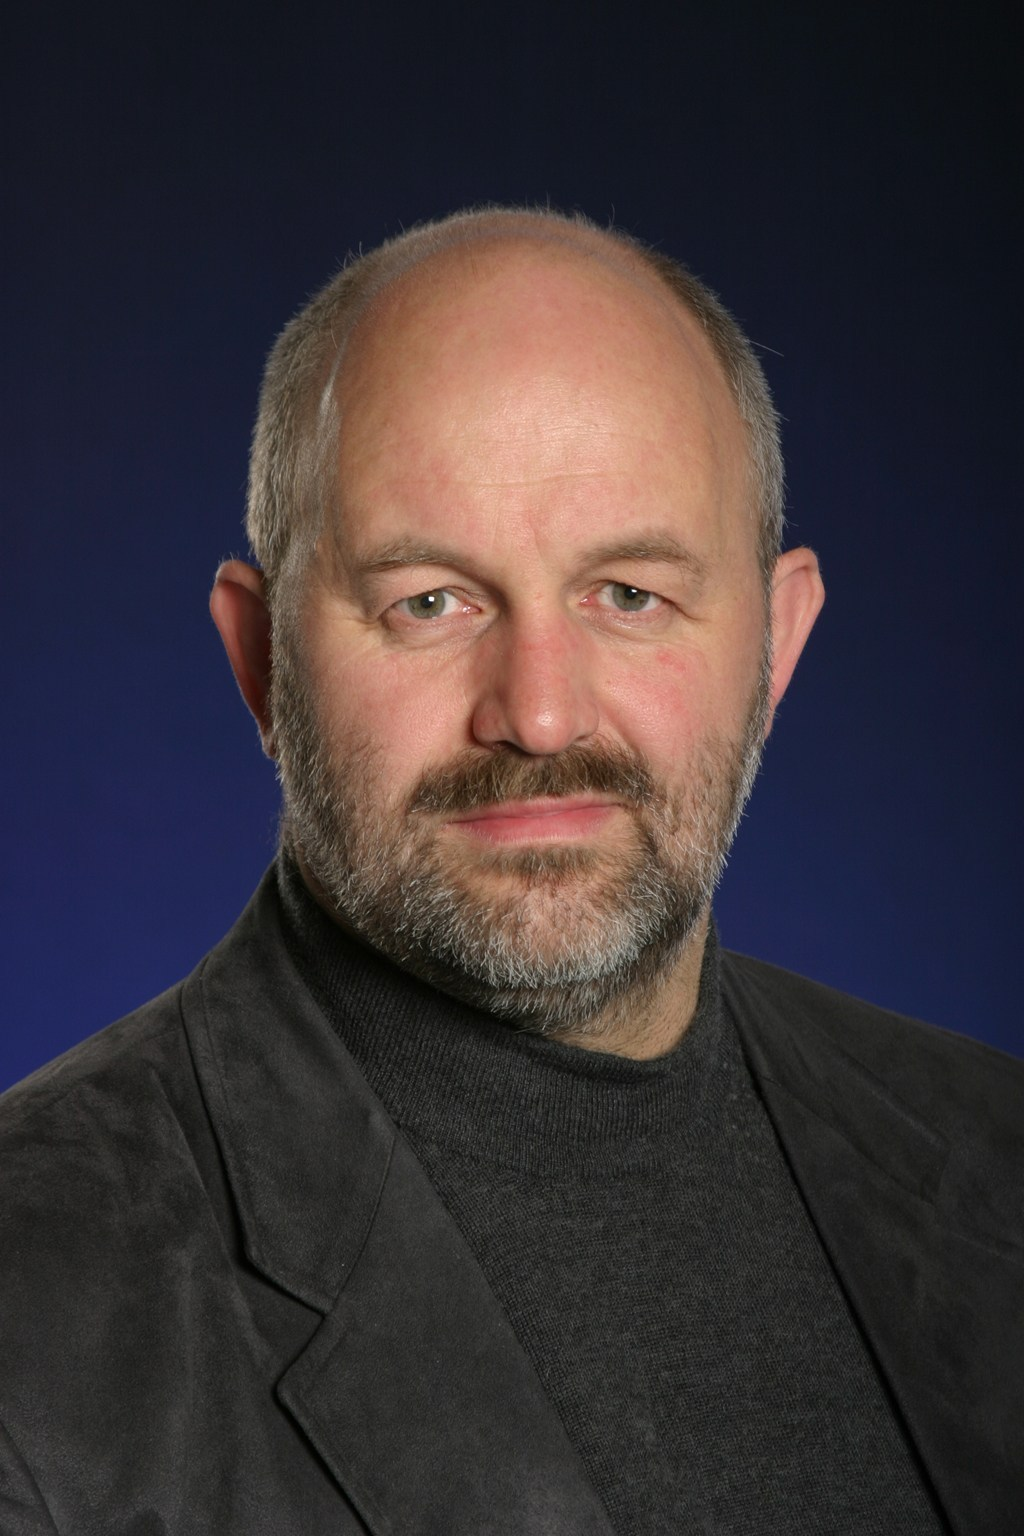
\includegraphics[
      width=0.22\textwidth,
      trim=0 75 0 25,
      clip
    ]{assets/vogels.jpg}
  };
}

\newcommand{\hoare}{
  \node[pic, right=0.2cm of vogels] (hoare) {
    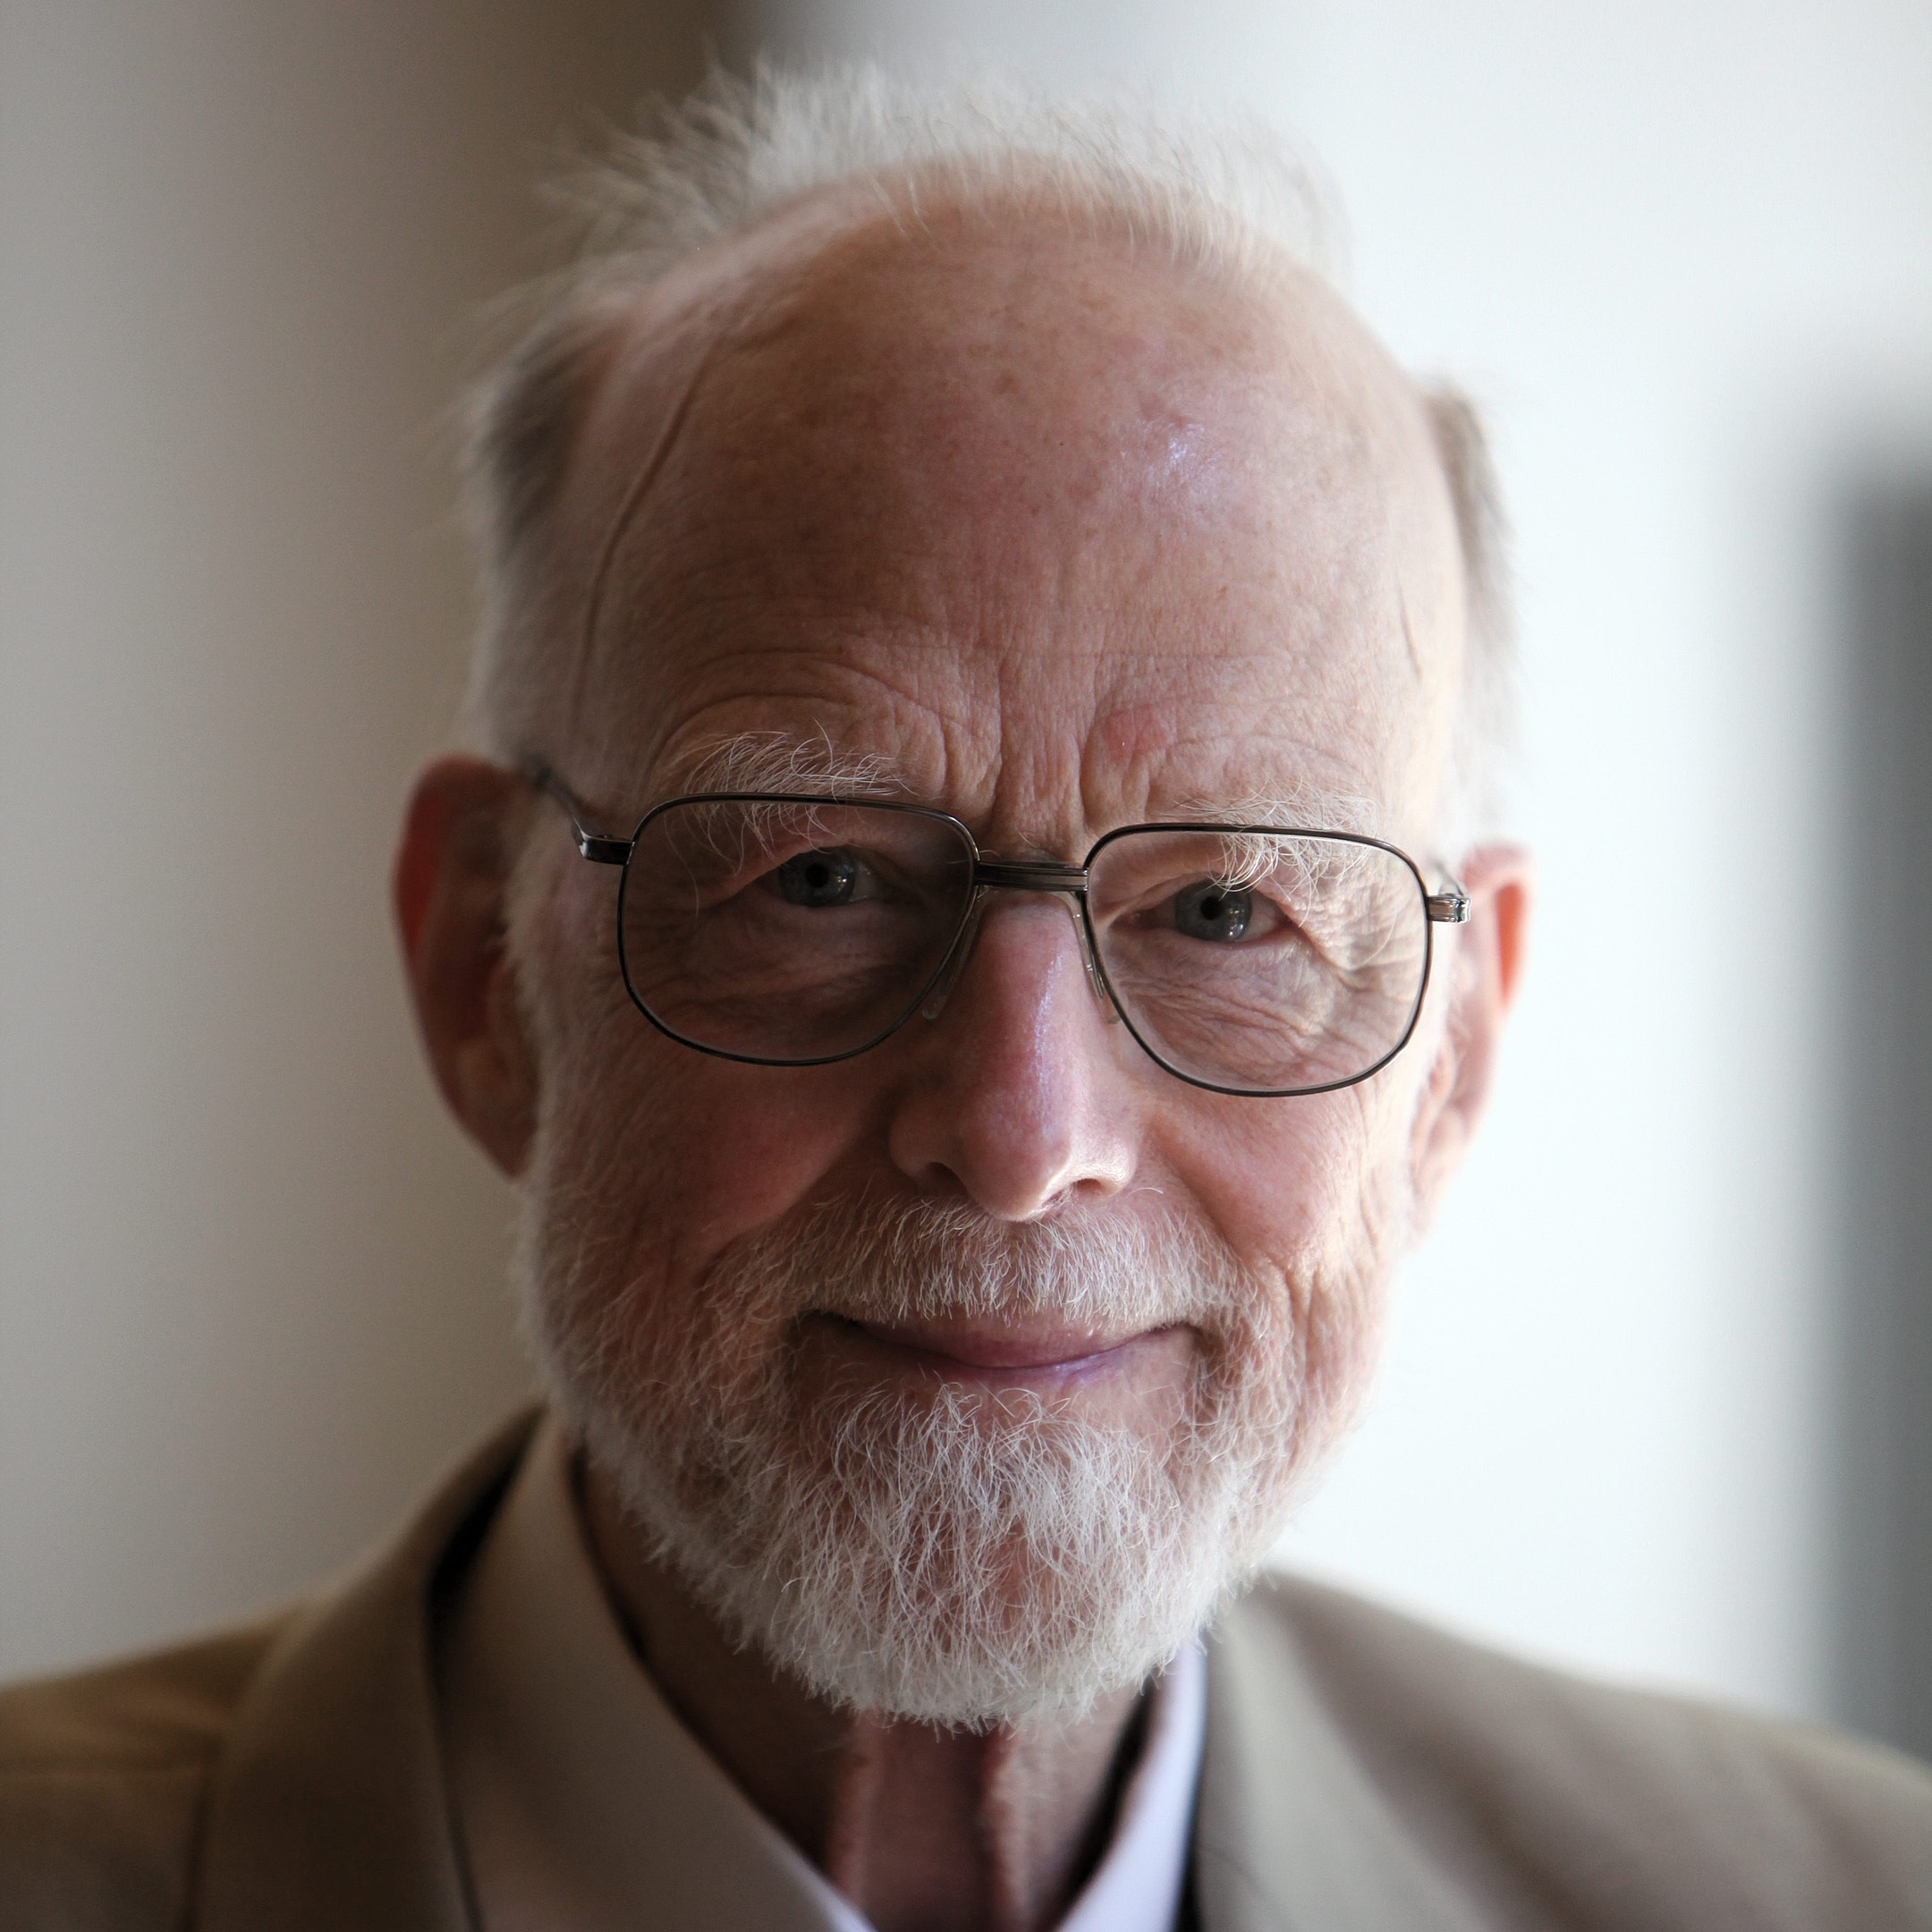
\includegraphics[width=0.22\textwidth]{assets/hoare.jpg}
  };
}

\newcommand{\lamport}{
  \node[pic, right=0.2cm of hoare] (lamport) {
    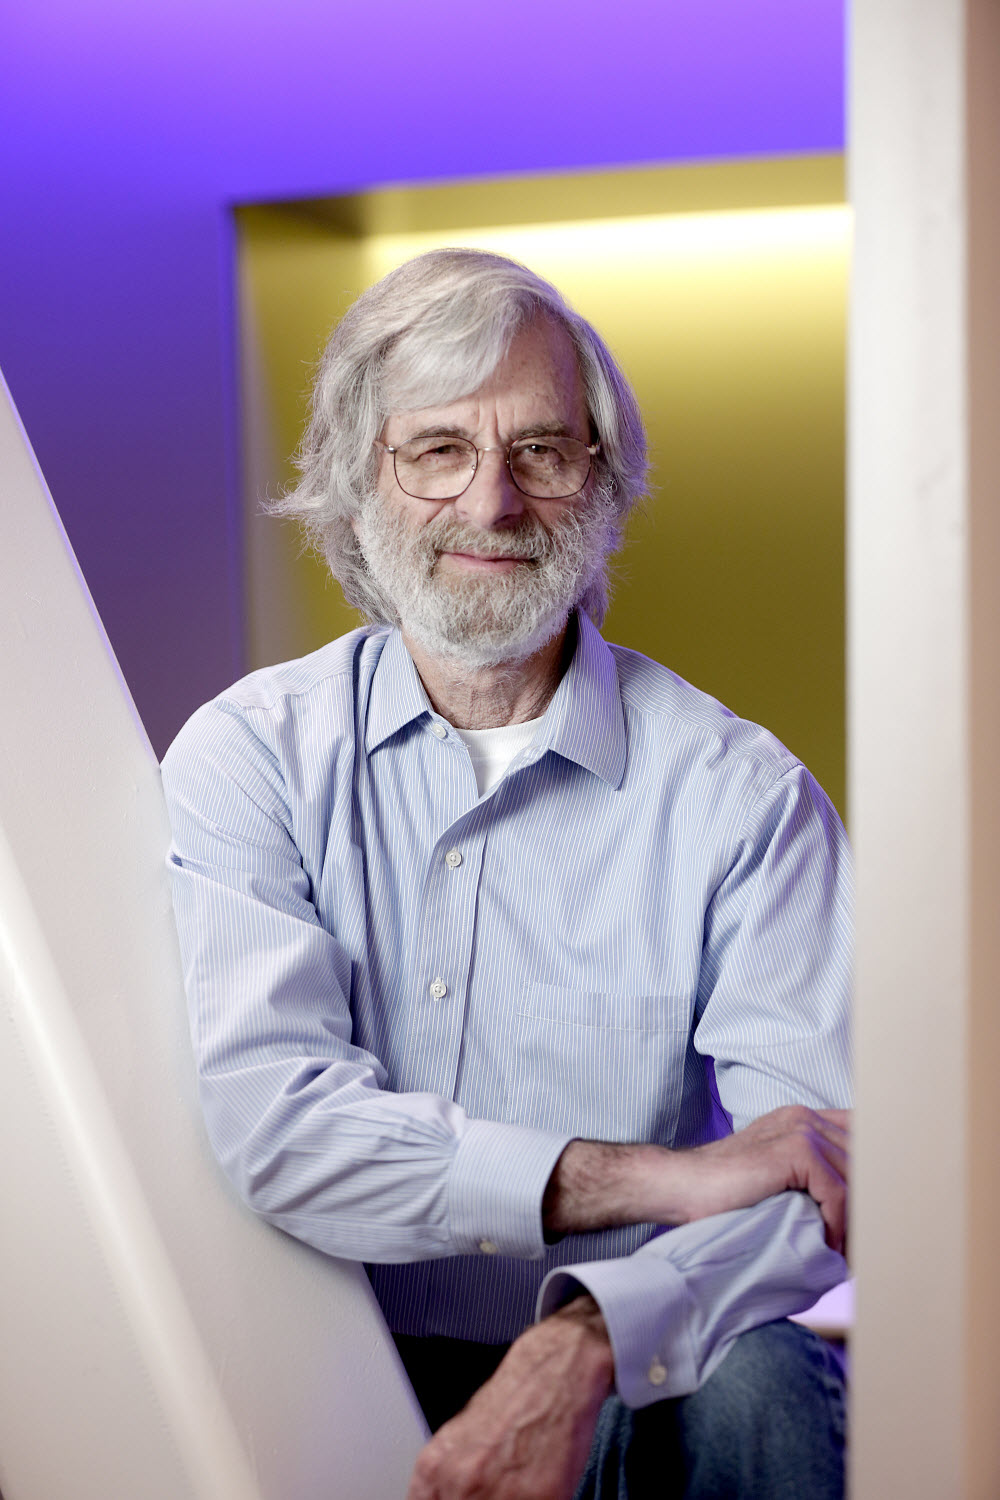
\includegraphics[
      width=0.22\textwidth,
      trim=250 700 300 200,
      clip
    ]{assets/lamport.jpg}
  };
}

\newcommand{\brewer}{
  \node[pic, right=0.2cm of lamport] (brewer) {
    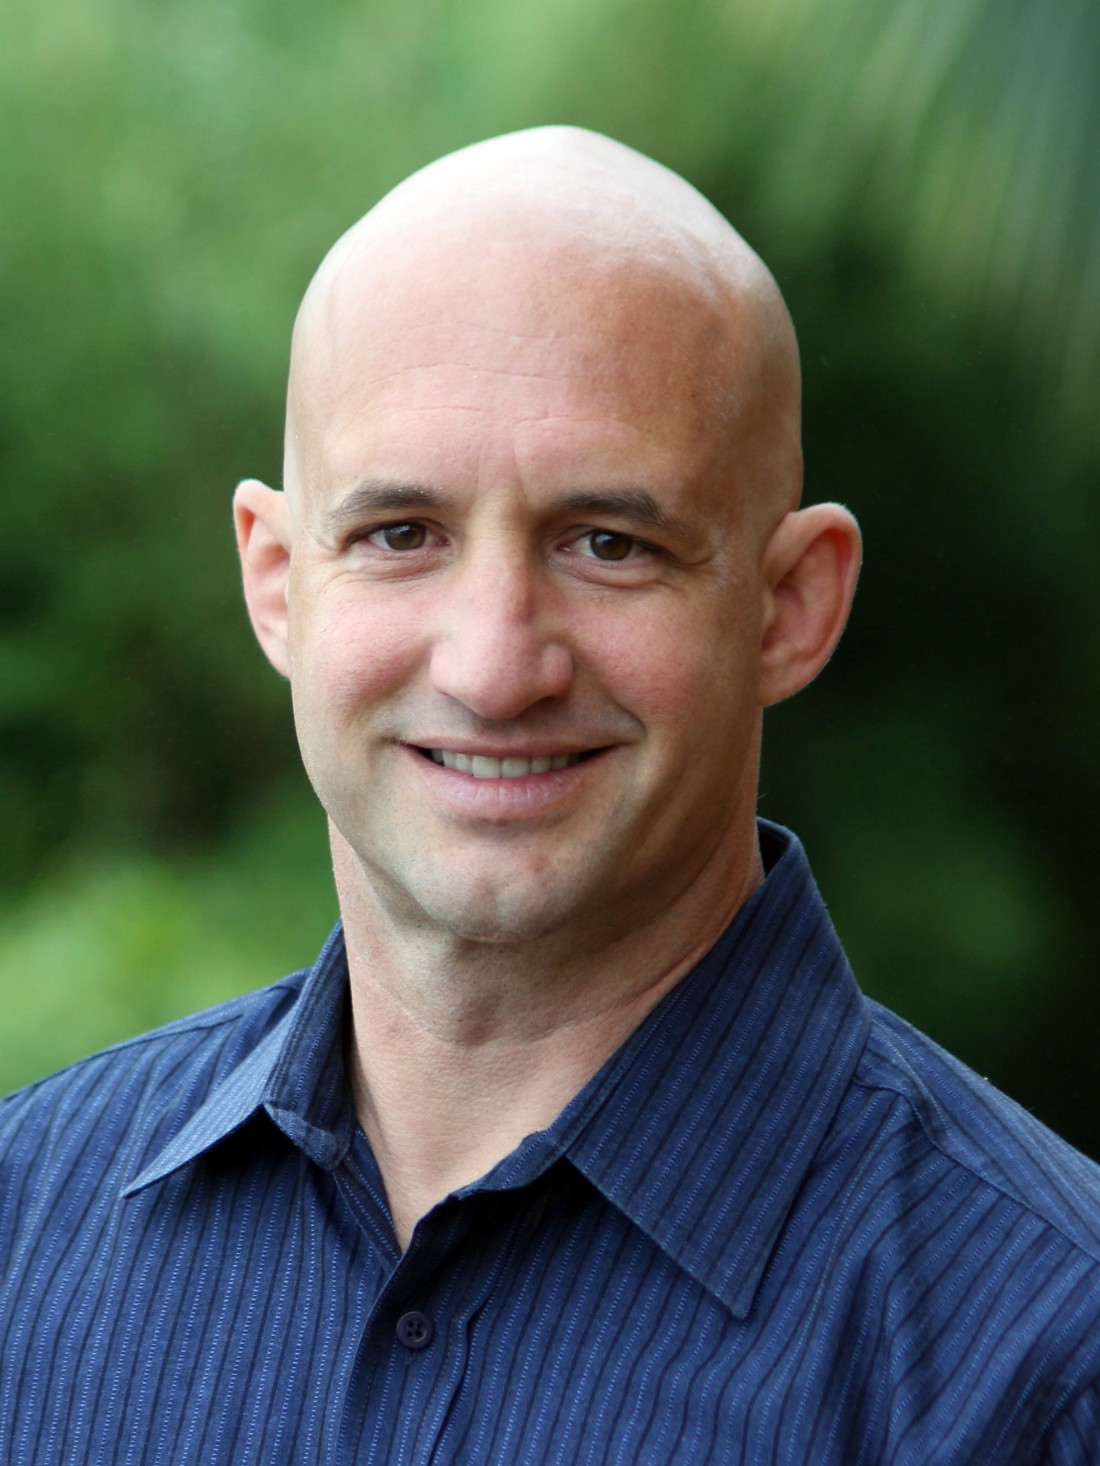
\includegraphics[
      width=0.22\textwidth,
      trim=100 300 100 100,
      clip
    ]{assets/brewer.jpg}
  };
}

\begin{frame}
  \note{%
    Hi everyone! Thanks so much for attending. I'm Michael, and today I'll be
    talking about ``Interactive Checks for Coordination Avoidance''. This is
    joint work with my advisor at UC Berkeley, Joe Hellerstein. \\[12pt]

    % I'd like to begin my talk with a short fairy tale. The fairy tale involves
    % an application developer who has some data they need to replicate.
    % Unfortunately, the application developer cannot decide whether to replicate
    % with weak consistency or strong consistency. The application developer
    % stays up all night trying to decide but eventually falls asleep at their
    % desk. In their sleep, they are visited by four wise men. And so, the fairy
    % tale begins:

    Imagine you're an application developer and you're trying to decide what
    kind of consistency you'd like to use to replicate some of your data.
  }
\end{frame}

\begin{frame}
  \begin{center}
    \begin{tikzpicture}[xscale=1.3]
      \vogels
      \node[quote, text width=0.8\textwidth, align=left] at (0, 3) {
        \Large\textit{
        Go with weak consistency. It's super duper fast and good enough for
        many applications!
        % Weak. Weak. It's weak that you're seeking.
        % \pause
        % Please learn that if you yearn your performance to peak, then turn no
        % further than weak.
      }
      };
      \path[fill=gray!30] (vogels.north) -- ++(0, 1) -- ++(0.5, 0) -- (vogels.north);
    \end{tikzpicture}
  \end{center}

  \note{%
    Someone like Werner Vogels would probably tell you to use weak consistency.
    You can implement weak consistency super duper fast, and for many
    applications, weak consistency is good enough. \\[12pt]

    % ``Weak. Weak. It's weak that you're seeking'', squeaked Werner Vogels.
    % His voice trembled, creaking, as he kept speaking.
    % ``Please learn that if you yearn your performance to peak,
    % then turn no further than weak.'' critiqued Werner.
    %
    % Werner Vogels has a good point. You can implement weak consistency super
    % duper fast, and for many applications, weak consistency is good enough.
    % But, let's continue.
  }
\end{frame}

\begin{frame}
  \begin{center}
    \begin{tikzpicture}[xscale=1.3]
      \vogels
      \hoare
      \node[quote, text width=0.8\textwidth, align=left] at (1, 3) {
        \Large\textit{
          Weakly consistent systems are so hard to reason about!
          % No. No. No more.
          % \pause
          % Weak is not easy. Weak is just treason. Please, these anomalies make
          % it so hard to reason.
        }
      };
      \path[fill=gray!30] (hoare.north) -- ++(0, 1) -- ++(0.5, 0) -- (hoare.north);
    \end{tikzpicture}
  \end{center}

  \note{%
    Tony Hoare would encourage us not to settle for weak consistency because a
    weakly consistent system is hard to reason about.

    % ``No, no, no more'' groaned Tony Hoare.
    % He moaned, he lamented, his soul was tormented
    % ``Weak is not easy. Weak is just treason.
    % Please, these anomalies, make it so hard to reason.''
    %
    % You see, Tony Hoare encourages us not to settle for weak consistency
    % because a weakly consistent system is very hard to reason about.
  }
\end{frame}

\begin{frame}
  \begin{center}
    \begin{tikzpicture}[xscale=1.3]
      \vogels
      \hoare
      \lamport
      \node[quote, text width=0.8\textwidth, align=left] at (2, 3) {
        \Large\textit{
          Go with a strongly consistent system! I think there are some good
          algorithms for that kind of stuff.
          % You see, I agree.
          % \pause
          % Weak is just wrong, not right for long. To defend your end users, you
          % must go with strong.
        }
      };
      \path[fill=gray!30] (lamport.north) -- ++(0, 0.5) -- ++(0.25, 0) -- (lamport.north);
    \end{tikzpicture}
  \end{center}

  \note{%
    Leslie Lamport would agree. He would encourage us to choose strong
    consistency. Strongly consistent systems are much easier to reason about.

    % ``You see, I agree'', says he, the ever mesmerizing Leslie.
    % ``Weak is just wrong, not right for long.
    % To defend your end users, you must go with strong.''
    %
    % Leslie Lamport encourages us to choose strong consistency becausesStrongly
    % consistent systems are much easier to reason about. After all a strongly
    % consistent system to end users looks exactly like a system that's not even
    % distributed.
  }
\end{frame}

\begin{frame}
  \begin{center}
    \begin{tikzpicture}[xscale=1.3]
      \vogels
      \hoare
      \lamport
      \brewer
      \node[quote, text width=0.8\textwidth, align=left] at (3, 3) {
        \Large\textit{
          Not so fast!
          % Alas, not so fast!
          % \pause
          % Consistency weak but not weary, strong but not nearly as fast as you
          % think when you hear my CAP theory.
        }
      };
      \path[fill=gray!30] (brewer.north) -- ++(0, 1) -- ++(-1, 0) -- (brewer.north);
    \end{tikzpicture}
  \end{center}

  \note{%
    Eric Brewer would counter that strong consistency isn't perfect. Strong
    consistency comes at the price of availability and performance. So we're in
    a bit of a pickle. Weak consistency is too confusing and strong consistency
    is too heavy handed.

    %
    % ``Alas, not so fast'', Brewer the dapper chap clapped back.
    % ``Consistency weak but not weary, strong but not nearly
    % as fast as you think when you hear my CAP theory.''
    %
    % Eric Brewer is right. Surely, strong consistency comes at the price of
    % availability and performance. So our application developer is in a bit of a
    % pickle. Weak consistency is too confusing and strong consistency is too
    % heavy handed. Fortunately, a hero emerges to save the day.
  }
\end{frame}

\begin{frame}
  \begin{center}
    \begin{tikzpicture}[xscale=1.3]
      \node[pic] (bailis) at (0, 0) {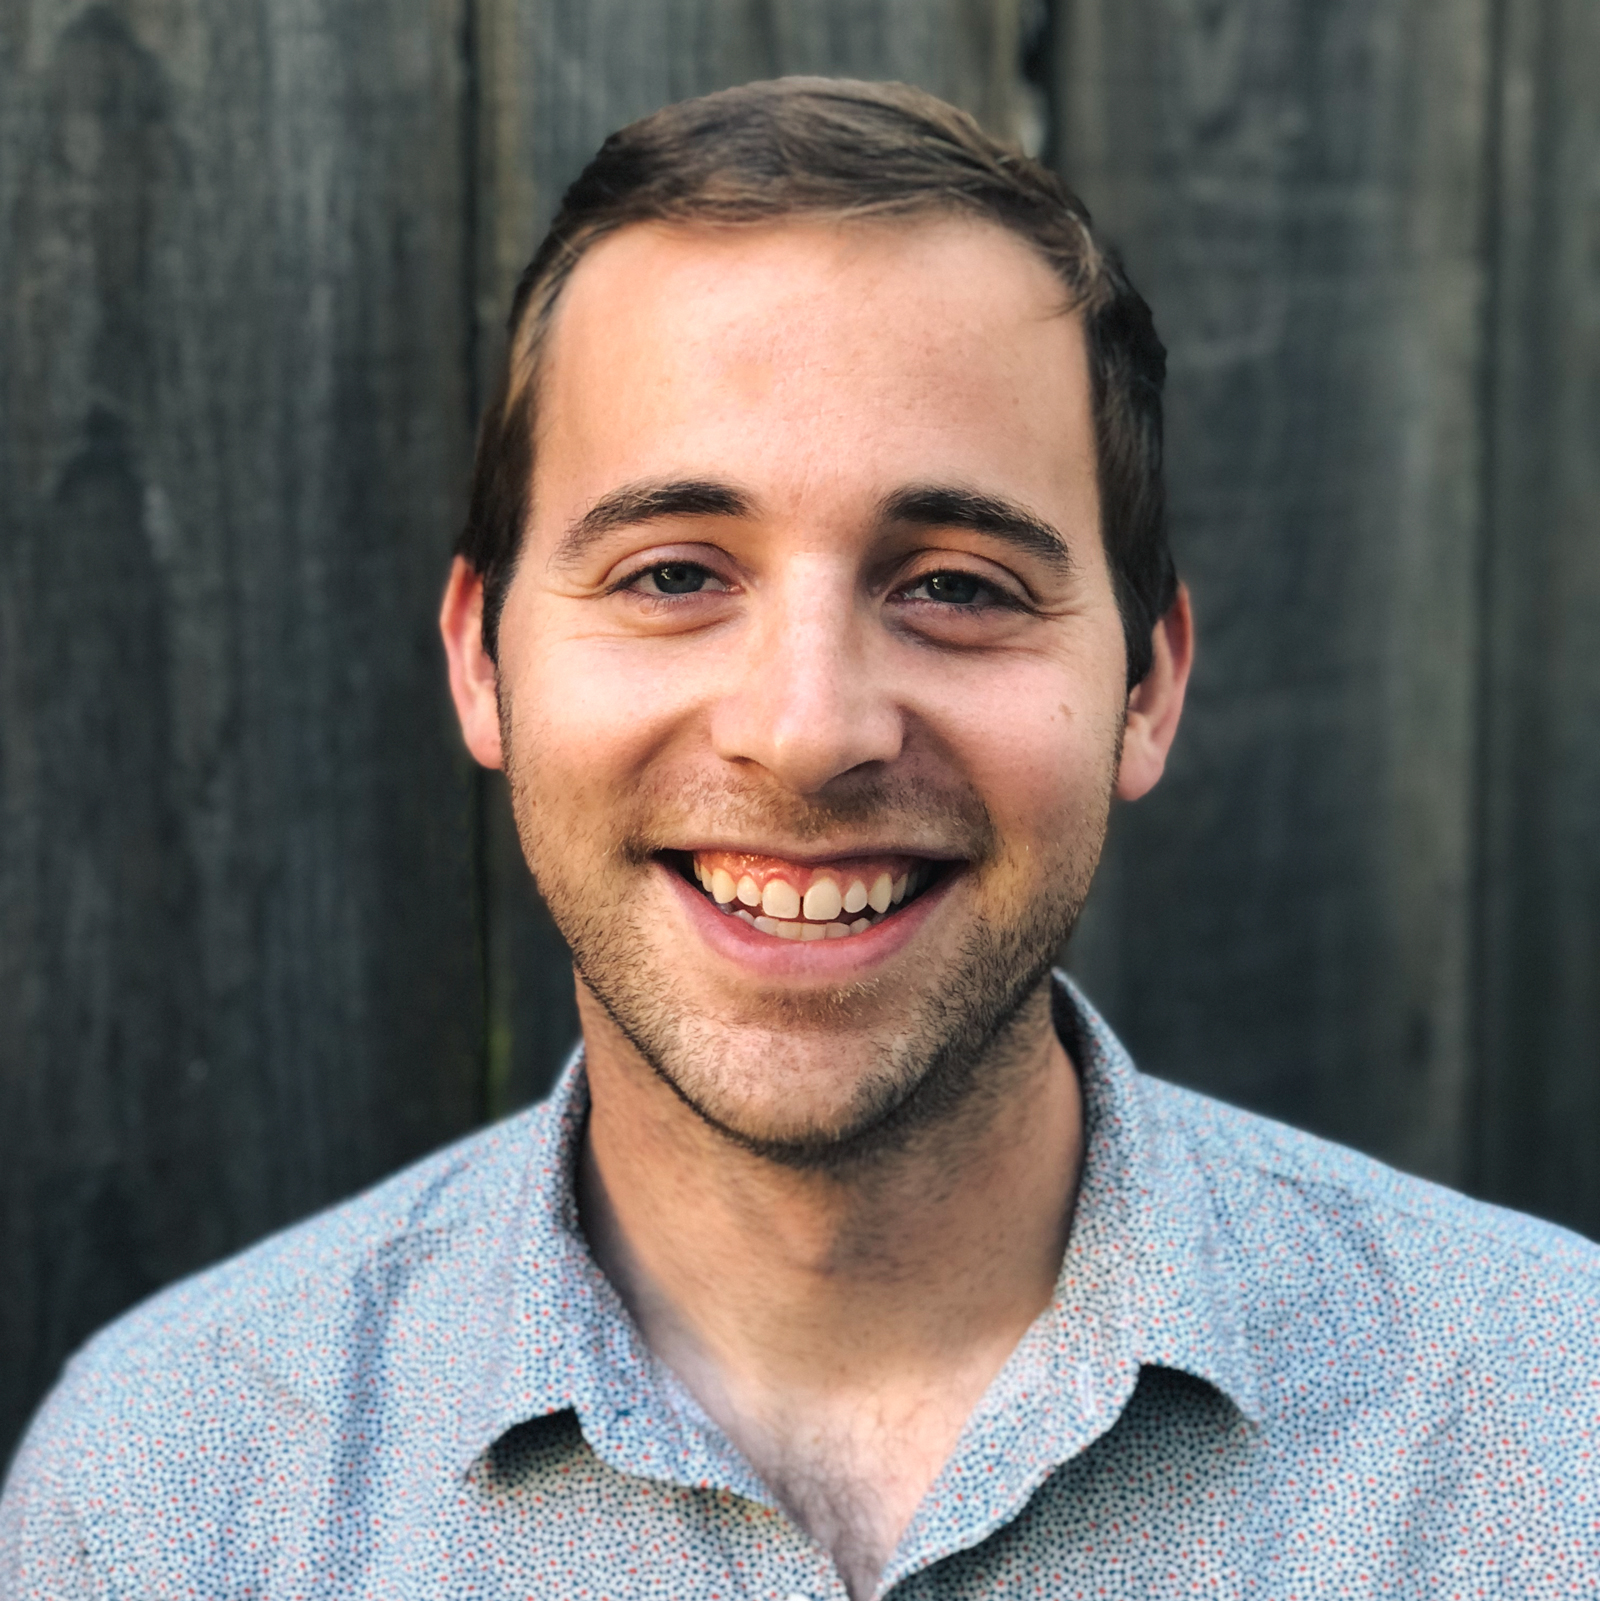
\includegraphics[width=0.25\textwidth]{assets/bailis.jpg}};
      \node[quote, text width=0.8\textwidth, align=left] at (0, 3) {
        \Large\textit{Why not have both?}
      };
      \path[fill=gray!30] (bailis.north) -- ++(0, 1.5) -- ++(1, 0) -- (bailis.north);
    \end{tikzpicture}
  \end{center}

  \note{%
    % Out teetered Peter, with swagger demeanor.
    % ``Why not have both?'' quoth the Peter.
    % The end.

    Fortunately, Peter Bailis can save the and reminding us of when in 2014, he
    and some other smart folks including Alan defined invariant confluence as a
    way to get the benefits of both weak and strong consistency.

    Invariant confluence will be the topic of this talk, so let's build some
    intuition on what invariant confluence is.
  }
\end{frame}
}
% {\newcommand{\bankdistance}{4}
\tikzstyle{bank}=[
  draw,
  minimum width=1.5cm,
  minimum height=1cm,
  font=\huge
]
\tikzstyle{op}=[
  -latex,
  ultra thick
]

\newcommand{\drawbanks}[6]{{
  \newcommand{\banka}{#1}
  \newcommand{\bankb}{#2}
  \newcommand{\bankaa}{#3}
  \newcommand{\bankbb}{#4}
  \newcommand{\bankaaa}{#5}
  \newcommand{\bankbbb}{#6}

  \node[bank, label=above:{Replica $A$}] (a1) at (0,              0) {\banka};
  \node[bank                           ] (a2) at (0,             -3) {\bankaa};
  \node[bank                           ] (a3) at (0,             -6) {\bankaaa};
  \node[bank, label=above:{Replica $B$}] (b1) at (\bankdistance,  0) {\bankb};
  \node[bank                           ] (b2) at (\bankdistance, -3) {\bankbb};
  \node[bank                           ] (b3) at (\bankdistance, -6) {\bankbbb};

  \draw[op] (a1) -- (a2);
  \draw[op] (a2) -- (a3);
  \draw[op] (b1) -- (b2);
  \draw[op] (b2) -- (b3);
}}

\newcommand{\zigzag}[2]{{
  \newcommand{\banka}{#1}
  \newcommand{\bankb}{#2}

  \draw[red, op] ($(\banka) + (0, -0.7)$) -- ($(\bankb) + (0, -1.0)$);
  \draw[red, op] ($(\bankb) + (0, -1.0)$) -- ($(\banka) + (0, -1.3)$);
  \draw[red, op] ($(\banka) + (0, -1.3)$) -- ($(\bankb) + (0, -1.6)$);
  \draw[red, op] ($(\bankb) + (0, -1.6)$) -- ($(\banka) + (0, -1.9)$);
}}

\begin{frame}{Replicated Bank Account}
  \begin{center}
    \begin{tikzpicture}
      \node[bank, label=above:{Replica $A$}] (a1) at (0, 0) {\$50};
      \node[bank, label=above:{Replica $B$}] (b1) at (\bankdistance, 0) {\$50};
    \end{tikzpicture}
  \end{center}

  \note{%
    We'll begin with an example.

    Let's say we want to replicate the database shown here. This database is
    the world's simplest database. It contains only a single number, which
    represents my bank account balance. We decide to replicate this database
    across two machines, replica A and replica B.

    Users can issue transactions to the database, and every transacation is
    either a deposit or a withdrawal. And, I have one critical invariant that I
    want to maintain over my database. And that invariant is that my bank
    account balance should never be negative. My balance must be non-negative at all times.
  }
\end{frame}

\begin{frame}{Coordinating}
  \begin{center}
    \begin{tikzpicture}
      \drawbanks{\$50}{\$50}
                {\$60}{\$60}
                {\$80}{\$80}

      \draw[op] ($(a1) + (-2, 0)$) -- (a1) node[midway, above] {$+\$10$};
      \draw[op] ($(b1) + (+2, 0)$) -- (b1) node[midway, above] {$+\$20$};
      \draw[op] (a2) -- ($(a2) + (-2, 0)$) node[midway, above] {OK};
      \draw[op] (b3) -- ($(b3) + (+2, 0)$) node[midway, above] {OK};

      \zigzag{a1}{b1}
      \zigzag{a2}{b2}
    \end{tikzpicture}
  \end{center}

  \note{%
    One way to replicate our database is by using coordination to implement
    strong consistency. For example, imagine a user issues a deposit of 10
    dollars to replica A, and simultaneously, a user issues a deposit of 20
    dollars to replica B. The two replicas can coordinate, for example by
    running Paxos, and agree on a single total order in which to execute the
    two transactions. Here, the replicas agree to deposit 10 dollars and then
    deposit 20 dollars. Both transactions succeed, and the replicas send back OK
    messages to the clients letting them know everything went smoothly.
  }
\end{frame}

\begin{frame}{Coordinating}
  \begin{center}
    \begin{tikzpicture}
      \drawbanks{\$50}{\$50}
                {\$20}{\$20}
                {\$20}{\$20}

      \draw[op] ($(a1) + (-2, 0)$) -- (a1) node[midway, above] {$-\$30$};
      \draw[op] ($(b1) + (+2, 0)$) -- (b1) node[midway, above] {$-\$40$};
      \draw[op] (a2) -- ($(a2) + (-2, 0)$) node[midway, above] {OK};
      \draw[op] (b3) -- ($(b3) + (+2, 0)$) node[midway, above] {NO};

      \zigzag{a1}{b1}
      \zigzag{a2}{b2}
    \end{tikzpicture}
  \end{center}

  \note{%
    Now, assume two clients issue concurrent withdrawal transactions of 30
    dollars and 40 dollars. Again, the two replicas coordinate and agree to
    execute the withdrawal of 30 dollars and then the withdrawal of 40 dollars.

    The withdrawal of 30 dollars executes fine, brining my bank account balance
    to 20 dollars, but the withdrawal of 40 dollars fails because I only have
    20 dollars left. So replica A sends back an OK message to the client, but
    replica B sends back a NO message letting the client know the transaction
    failed. And while the transaction failed, you'll note that we never
    violated our application invariant.
  }
\end{frame}

\begin{frame}{Avoiding Coordination}
  \begin{center}
    \begin{tikzpicture}
      \drawbanks{\$50}{\$50}
                {\$60}{\$70}
                {\$80}{\$80}

      \draw[op] ($(a1) + (-2, 0)$) -- (a1) node[midway, above] {$+\$10$};
      \draw[op] ($(b1) + (+2, 0)$) -- (b1) node[midway, above] {$+\$20$};
      \draw[op] (a2) -- ($(a2) + (-2, 0)$) node[midway, above] {OK};
      \draw[op] (b2) -- ($(b2) + (+2, 0)$) node[midway, above] {OK};

      \draw[dashed, op] (a2) -- (b3) node[near start, sloped, above] {$+\$10$};
      \draw[dashed, op] (b2) -- (a3) node[near start, sloped, above] {$+\$20$};
    \end{tikzpicture}
  \end{center}

  \note{%
    Alternatively, instead of implementing our bank with strong consistency, we
    could implement it with weak consistency and avoid coordination altogether.

    Now, when two clients issue concurrent deposit transactions, the two
    replicas execute the transactions immediately without consulting one
    another. And every once in a while, the two replicas communicate and fill
    each other in on the transactions they missed.

    Here, for example, replica A lets replica B know to deposit 10 dollars and
    replica B lets replica A know to deposit 20 dollars. Notice that even
    though we didn't perform any coordination, the two replicas never violate
    my critical invariant of a non-negative balance.
  }
\end{frame}

\begin{frame}{Avoiding Coordination}
  \begin{center}
    \begin{tikzpicture}
      \drawbanks{\$50}{\$50}
                {\$20}{\$10}
                {-\$20}{-\$20}

      \draw[op] ($(a1) + (-2, 0)$) -- (a1) node[midway, above] {$-\$30$};
      \draw[op] ($(b1) + (+2, 0)$) -- (b1) node[midway, above] {$-\$40$};
      \draw[op] (a2) -- ($(a2) + (-2, 0)$) node[midway, above] {OK};
      \draw[op] (b2) -- ($(b2) + (+2, 0)$) node[midway, above] {OK};

      \draw[dashed, op] (a2) -- (b3) node[near start, sloped, above] {$-\$30$};
      \draw[dashed, op] (b2) -- (a3) node[near start, sloped, above] {$-\$40$};
    \end{tikzpicture}
  \end{center}

  \note{%
    However, let's look what happens when two clients issue concurrent
    withdrawals. Both withdrawals are executed locally and both succeed.
    However, when the two replicas exchange transactions with one another, they
    both enter an invariant violating state of negative twenty dollars!
  }
\end{frame}

\begin{frame}
  \begin{center}
    \Huge
    Deposits don't require coordination to maintain invariants, but withdrawals
    do.
  \end{center}

  \note{%
    We can learn a lot from these examples.

    First, if we implement our bank with strong consistency, we never violate
    our invariant.

    Second, we can implement deposit transactions without any coordination and
    we're still guaranteed to never violate the invariant.

    Third, withdrawal transactions, unlike deposit transactions, do require
    coordination to avoid violating the invariant.

    At a very high level, invariant confluence tries to capture exactly which
    transactions require coordination to maintain invariants and which do not.
    In this example, deposit transactions are invariant confluent and thus do
    not require coordination while withdrawal transactions are not invariant
    confluent and thus do require coordination.
  }
\end{frame}
}
{\section{\Iconfluence{}}
In this section, we present six different ways to think about \Iconfluence{}:
three state-based approaches and three operation-based approaches.

\subsection{State-Based}
\begin{definition}
  A \defword{distributed state-based object} is a triple $(S, s_0, \join)$
  where $S$ is a set of states, $s_0 \in S$ is a designated start state, and
  $\join: S \times S \to S$ is a binary merge operator that we call join.
\end{definition}

The notion of state-based objects is taken from~\cite{shapiro2011conflict}.
Note that $\join$ is an \emph{arbitrary} function. It does not necessarily have
to satisfy any special properties like associativity or commutativity, though
later we will see that often it does.

\begin{definition}
  A \defword{state-based transaction} $t: S \to S$ is a function that maps one
  state to another.
\end{definition}

\begin{definition}
  An \defword{invariant} $I \subseteq S$ is a subset of states. Notationally,
  we say $I(s)$ to mean $s \in I$ and $\lnot I(s)$ to mean $s \notin I$.
\end{definition}

\begin{example}
  $(\nats, 0, +)$ is a distributed object, $t(x) = 2x$ is a transaction, and
  $\setst{x \in \nats}{x \equiv 0 \mod 2}$ is an invariant. Here, $I(0)$ and
  $I(2)$ but $\lnot I(1)$ and $\lnot I(3)$.
\end{example}

There are three ways to think about state-based \Iconfluence{}: a process-based
approach, a graph-based approach, and an expression-based approach. All three
approaches are illustrated in \figref{statebasedmodels} and are described in
more detail below.

\input{figs/statebased_iconfluence.fig}

\subsubsection{Process-Based}
The process-based model is most similar to the process model described by
Shapiro et al.\ in~\cite{shapiro2011conflict}. We are given a set
$\seq{p}{1}{n}$ of $n$ processors each of which begins with state $s_0$.  A
processor $p_i$ can perform one of two actions.

First, $p_i$ can execute a transaction $t \in T$ to transition from state $s$
to state $t(s)$, given that $I(t(s))$. If $\lnot I(t(s))$, then $p_i$ will not
execute $t$ (or it will execute $t$ but then abort it; think of it however you
like).

Second, $p_i$ can send its state $s_i$ to another processor $p_j$ with state
$s_j$ causing $p_j$ to transition from state $s_j$ to state $s_i \join s_j$ (or
$s_j \join s_i$; it doesn't really matter). Note that unlike executing a
transaction, $p_j$ must transition from $s_j$ to $s_i \join s_j$ even if $\lnot
I(s_i \join s_j)$.

$T$ is invariant-confluent with respect to $I$, abbreviated \Iconfluent{}, if
every reachable state (including $s_0$) satisfies the invariant. Note that this
definition of \Iconfluence{} is different from the original definition
in~\cite{bailis2014coordination}. Later, we will see that they are equivalent.

\subsubsection{Graph-Based}
The graph-based approach is most similar to the model used by Bailis et al.\
in~\cite{bailis2014coordination}. We are given a directed acyclic graph where
vertices are states, and edges are either labelled with transactions or are
unlabelled if they correspond to a join. The graph is really just an alternate
way of representing an execution in the process-based model, but with duplicate
states collapsed into a single vertex. As with the process-based model, we say
that $T$ is \Iconfluent{} if every vertex in every graph satisfies the
invariant.

\subsubsection{Expression-Based}
The expression-based approach formalizes the process-based and graph-based
approach using expressions. Given a state based object $(S, s_0, \join)$ and a
set of transactions $T$, we consider expressions generated by the following
grammar:
\[
  e ::= s_0 \mid t(e) \mid e_1 \join e_2
\]
where $t$ corresponds to a transaction in $T$. We can evaluate an expression
$e$, written $eval(e)$, in the obvious way:
\begin{mathpar}
  eval(s_0) \defeq s_0

  eval(t(e)) \defeq t(eval(e))

  eval(e_1 \join e_2) \defeq eval(e_1) \join eval(e_2)
\end{mathpar}

\begin{definition}
  An expression $e$ \defword{satisfies $I$}, denoted $I(e)$, if $I(eval(e))$.
\end{definition}

\begin{definition}
  Intuitively, we say an expression is \defword{reachable} if it can be reached
  in an execution of the process-based model. Formally, we defined a predicate
  $\reachable{\cdot}$ as follows:

  \begin{mathpar}
    \inferrule{ }{\reachable{s_0}}

    \inferrule{\reachable{e} \\ I(t(e))}{\reachable{t(e})}

    \inferrule{\reachable{e_1} \\ \reachable{e_2}}{\reachable{e_1 \join e_2}}
  \end{mathpar}
\end{definition}

\begin{definition}
  $T$ is \defword{\Iconfluent{}} if $\setst{e}{\reachable{e}} \subseteq I$. In
  other words, $T$ is \Iconfluent{} if all reachable states satisfy the
  invariant.
\end{definition}

As we mentioned earlier, this definition of \Iconfluence{} is different than
the original definition presented in~\cite{bailis2014coordination} (though it
is the same as the definition in~\cite{gotsman2016cause}), but they are
(almost) equivalent. We introduce some definitions and then prove this.

\begin{definition}
  An expression \defword{recursively satisfies $I$}, denoted $\Irec{e}$, if $e$
  and all of $e$'s children satisfy $I$. That is,
  \begin{mathpar}
    \Irec{s_0} \defeq I(s_0)

    \Irec{t(e)} \defeq I(t(e)) \land \Irec{e}

    \Irec{e_1 \join e_2}
    \defeq I(e_1 \join e_2) \land \Irec{e_1} \land \Irec{e_2}
  \end{mathpar}
\end{definition}

Bailis et al.\ defined \Iconfluence{} to mean that expressions recursively
satisfying $I$ are closed under join. That is, $T$ is \Iconfluent{} if
\[
  \forall e_1, e_2.\; \Irec{e_1} \land \Irec{e_2} \implies I(e_1 \join e_2)
\]
If $\lnot I(s_0)$, then \Iconfluence{} holds vacuously which is a bit silly, so
Bailis et al.\ probably ought to have also added the condition $I(s_0)$ to
their definition of \Iconfluence{}. Doing so, the two definitions become
equivalent.

\begin{claim}\clmlabel{StateBasedIrecImpliesReachable}
  $\Irec{e} \implies \reachable{e}$
\end{claim}
\begin{elidableproof}
  We perform structural induction on $e$.
  \begin{itemize}
    \item \textbf{Case $s_0$.}
      Axiomatically, $\reachable{s_0}$.

    \item \textbf{Case $t(e)$.}
      $\Irec{t(e)}$, so $I(t(e))$ and $\Irec{e}$. By the inductive hypothesis,
      $\reachable{e}$, so by the definition of $\reachable{\cdot}$,
      $\reachable{t(e)}$.

    \item \textbf{Case $e_1 \join e_2$.}
      $\Irec{t(e)}$, so $\Irec{e_1}$ and $\Irec{e_2}$. By the inductive
      hypothesis, $\reachable{e_1}$ and $\reachable{e_2}$, so by the definition
      of $\reachable{\cdot}$, $\reachable{e_1 \join e_2}$.
  \end{itemize}
\end{elidableproof}

\begin{claim}\clmlabel{StateBasedTwoIconfluenceDefs}
  Consider a state based object $(S, s_0, \join)$, a set of transactions $T$,
  and an invariant $I$. The following two are equivalent:
  \begin{enumerate}[\quad(1)]
    \item
      $\setst{e}{\reachable{e}} \subseteq I$

    \item
      $I(s_0)$ and $\Irec{e_1} \land \Irec{e_2} \implies I(e_1 \join e_2)$
  \end{enumerate}
\end{claim}
\begin{elidableproof}
  First, we show that (1) implies (2). Axiomatically, $\reachable{s_0}$, so by
  (1), $I(s_0)$. Let $e_1$ and $e_2$ be arbitrary expressions such that
  $\Irec{e_1}$ and $\Irec{e_2}$. By \clmref{StateBasedIrecImpliesReachable},
  $\reachable{e_1}$ and $\reachable{e_2}$. Thus, $\reachable{e_1 \join e_2}$,
  so by (1), $I(e_1 \join e_2)$.

  Next, we show that (2) implies (1). We prove by structural induction that for
  all $e$, $\reachable{e} \implies \Irec{e}$. From this, (1) is immediate.
  \begin{itemize}
    \item \textbf{Case $s_0$.}
      $I(s_0)$ by (2), so $\Irec{s_0}$

    \item \textbf{Case $t(e)$.}
      $\reachable{t(e)}$, so $\reachable{e}$ and $I(t(e))$. By the inductive
      hypothesis, $\Irec{e}$, so by the definition of $\Irec{\cdot}$,
      $\Irec{t(e)}$.

    \item \textbf{Case $e_1 \join e_2$.}
      $\reachable{e_1 \join e_2}$, so $\reachable{e_1}$ and $\reachable{e_2}$.
      By the inductive hypothesis, $\Irec{e_1}$ and $\Irec{e_2}$. By $(2)$,
      $I(e_1 \join e_2)$. Thus, $\Irec{e_1 \join e_2}$.
  \end{itemize}
\end{elidableproof}

\subsection{Operation-Based}
\begin{definition}
  A \defword{distributed operation-based object} is a pair $(S, s_0)$ where $S$
  is a set of states and $s_0 \in S$ is a designated start state.
\end{definition}

Like state-based objects, the notion of operation-based objects is taken
from~\cite{shapiro2011conflict}. Note that we do not have a join function like
we did with state-based objects.

\begin{definition}
  An \defword{operation-based transaction} $t: S \to (S \to S)$ is a function
  that maps a state to a \defword{shadow transaction} $t(s): S \to S$. The term
  shadow transaction is taken from~\cite{li2014automating}.
\end{definition}

The definition of an invariant is the same in the state-based and
operation-based model.

\begin{example}
  $(\nats, 0)$ is a distributed object. $t(x) = y \mapsto x + y$ is a
  transaction that given a state $x$ returns a function $y \mapsto x + y$ that
  adds $x$ to its argument. $\setst{x \geq 0}{x \in \nats}$ is an invariant.
\end{example}

As with state-based objects, there are three ways to think about
operation-based \Iconfluence{}: a process-based approach, a graph-based
approach, and an expression-based approach. All three approaches are
illustrated in \figref{OpBasedModels} and are described in more detail below.

\input{figs/opbased_iconfluence.fig}

\subsubsection{Process-Based}
As with the state-based approach, the process-based model is most similar to
the process model described by Shapiro et al.\ in~\cite{shapiro2011conflict}.
We are given a set $\seq{p}{1}{n}$ of $n$ processors each of which begins with
state $s_0$. A processor $p_i$ can do one of two things.

First, $p_i$ can execute a transaction $t$ on its current state $s$ and then
transitions from state $s$ to state $t(s)(s)$, given that $I(t(s)(s))$. If
$\lnot I(t(s)(s))$, then $p_i$ will not perform $t$. If $p_i$ does execute $t$,
then it broadcasts $t(s)$ to all other processors exactly once.

Second, $p_i$ can receive a broadcasted shadow transaction $t(s_j)$ from some
other processor $p_j$. When $p_i$ receives $t(s_j)$, it transitions from its
state $s_i$ to state $t(s_j)(s_i)$. When $p_i$ receives a shadow transaction,
it must execute it, even if $\lnot I(t(s_j)(s_i))$.

$T$ is \Iconfluent{} if every reachable state (including $s_0$) satisfies the
invariant.

\subsubsection{Graph-Based}
In the graph-based model, we are given a directed acyclic graph in which each
vertex is a state $s$ and each edge is labelled with a shadow operation $t(s)$
where $s$ is some other vertex in the graph. $T$ is \Iconfluent{} if every
vertex in every graph satisfies $I$.

\subsubsection{Expression-Based}
Given an operation-based object $(S, s_0)$ and a set of transactions $T$, we
consider expressions built from the following grammar:
\[
  e ::= s_0 \mid t(e_1)(e_2)
\]
where $t$ corresponds to a transaction in $T$. We can evaluate an expression,
denoted $eval(e)$, in the obvious way:
\begin{mathpar}
  eval(s_0) \defeq s_0

  eval(t(e_1)(e_2)) \defeq t(eval(e_1))(eval(e_2))
\end{mathpar}

\begin{definition}
  An expression $e$ \defword{satisfies $I$}, denoted $I(e)$, if $I(eval(e))$.
\end{definition}

\begin{definition}
  As with state-based expressions, we formalize which operation-based
  expressions are reachable.

  \begin{mathpar}
    \inferrule{ }{\reachable{s_0}}

    \inferrule{
      \reachable{e_1} \\
      \reachable{e_2} \\
      I(t(e_1)(e_1))
    }{\reachable{t(e_1)(e_2)}}
  \end{mathpar}
\end{definition}

\begin{definition}
  $T$ is \Iconfluent{} if $\setst{e}{\reachable{e}} \subseteq I$.
\end{definition}

As with state-based objects, we have an equivalent definition of \Iconfluence{}
that deals with the closure of recursively invariant satisfying states.

\begin{definition}
  An expression \defword{recursively satisfies $I$}, denoted $\Irec{e}$, if $e$
  and all of $e$'s children satisfy $I$. That is,
  \begin{mathpar}
    \Irec{s_0} \defeq I(s_0)

    \Irec{t(e_1)(e_2)} \defeq I(t(e_1)(e_2)) \land \Irec{e_1} \land \Irec{e_2}
  \end{mathpar}
\end{definition}

\begin{claim}\clmlabel{OpBasedIrecImpliesReachable}
  $\Irec{e} \implies \reachable{e}$
\end{claim}
\begin{elidableproof}
  We perform a structural induction on $e$.
  \begin{itemize}
    \item \textbf{Case $s_0$.}
      Axiomatically, $\reachable{s_0}$.

    \item \textbf{Case $t(e_1)(e_2)$.}
      $\Irec{t(e_1)(e_2)}$, so $\Irec{e_1}$, $\Irec{e_2}$, and
      $I(t(e_1)(e_1))$. By the inductive hypothesis, $\reachable{e_1}$ and
      $\reachable{e_2}$. Thus, $\reachable{t(e_1)(e_2)}$.
  \end{itemize}
\end{elidableproof}

\begin{claim}\clmlabel{OpBasedTwoIconfluenceDefs}
  Given an operation-based object $(S, s_0)$, a set of transactions $T$, and an
  invariant $I$, the following two are equivalent:
  \begin{enumerate}[\quad(1)]
    \item
      $\setst{e}{\reachable{e}} \subseteq I$

    \item
      $I(s_0)$ and $\Irec{e_1} \land \Irec{e_2} \land I(t(e_1)(e_1)) \implies
      I(t(e_1)(e_2))$.
  \end{enumerate}
\end{claim}
\begin{elidableproof}
  First, we show that (1) implies (2). $\reachable{s_0}$, so by (1), $I(s_0)$.
  Let $e_1$ and $e_2$ be arbitrary expressions such that $\Irec{e_1}$,
  $\Irec{e_2}$, and $I(t(e_1)(e_1))$. By \clmref{OpBasedIrecImpliesReachable},
  $\reachable{e_1}$ and $\reachable{e_2}$, so $\reachable{t(e_1)(e_2)}$. By
  (1), $I(t(e_1)(e_2))$.

  Next, we show that (2) implies (1). We show by structural induction on $e$
  that $\reachable{e} \implies \Irec{e}$. From this, (1) is immediate.
  \begin{itemize}
    \item \textbf{Case $s_0$.}
      By (2), $I(s_0)$, so $\Irec{s_0}$.

    \item \textbf{Case $t(e_1)(e_2)$.}
      $\reachable{t(e_1)(e_2)}$, so $\reachable{e_1}$, $\reachable{e_2}$, and
      $I(t(e_1)(e_1))$. By the inductive hypothesis, $\Irec{e_1}$ and
      $\Irec{e_2}$. By (2), $I(t(e_1)(e_2))$, so $\Irec{t(e_1)(e_2)}$.
  \end{itemize}
\end{elidableproof}
}
% {\begin{frame}
  \Huge
  \begin{center}
    Goal: develop an invariant-confluence decision procedure.
  \end{center}

  \note{%
    Now that we've defined invariant confluence, we can turn our attention to
    the main goal of our paper. And that is to develop an invariant-confluence
    decision procedure. Determining whether or not a distributed object is
    invariant confluent is not easy to do by hand, so we'd like to develop a
    decision procedure that can automatically check whether something is
    invariant confluent for us.
  }
\end{frame}

\begin{frame}
  \Huge
  \begin{center}
    Reasoning about reachable states is hard.
  \end{center}

  \note{%
    Unfortunately, developing an invariant confluence decision procedure
    straight up is not easy. Invariant confluence is fundamentally a property
    about reachable states but reasoning automatically about reachable states
    is hard.

    Instead of reasoning about invariant confluence directly then, let's look
    at a sufficient condition for invariant confluence called invariant
    closure.
  }
\end{frame}

\begin{frame}
  \Large
  We say a set $S$ is \defword{closed under $f$} if for every $x, y \in S, f(x,
  y) \in S$. \pause For example,
  \begin{itemize}
    \item Even numbers are closed under addition.
    \item Odd numbers are \emph{not} closed under addition.
  \end{itemize}

  \note{%
    First, a quick refresher on what it meas for a set to be closed. We say a
    set $S$ is closed under a binary operator $f$ if for every $x$ and $y$ in
    $S$, $f(x, y)$ is also in $S$. For example, even numbers are closed under
    addition because the sum of any two even numbers is even. But odd numbers
    are not closed under addition because the sum of two odd numbers may not
    be odd.
  }
\end{frame}

\begin{frame}
  \Large
  $O = (S, \join)$ is \defword{\invariantclosed{}} with respect to an invariant
  $I$, abbreviated \defword{\Iclosed{}}, if invariant satisfying states are
  closed under merge. \pause That is, for every state $s_1, s_2 \in S$, if
  $I(s_1)$ and $I(s_2)$, then $I(s_1 \join s_2)$.

  \note{%
    We say that an object $O$ is invariant closed if invariant satisfying
    states are closed under merge. That is, if an object is invariant closed,
    then for every pair of states $s_1$ and $s_2$, if $s_1$ and $s_2$ satisfy
    the invariant then so does $s_1 \join s_2$.
  }
\end{frame}

\begin{frame}
  \Large
  \[
    \text{invariant closure} \implies \text{invariant confluence}
  \]
  \pause
  Transactions perserve invariants. If merging does too, then all reachable
  states satisfy the invariant.

  \note{%
    Invariant closure is a sufficient condition for invariant confluence. Why
    is that? Well for an object to be invariant confluent, every reachable
    state must satisfy the invariant. A state is reachable if it can be reached
    by executing transactions merging states. Transactions are already
    guarnateed to preserve invariants, so if merging is also guaranteed to
    preserve the invariant, then every reachable state always satisfies the
    invariant.
  }
\end{frame}

\begin{frame}
  \Large
  Checking invariant closure is more straightforward.
  \pause
  \begin{align*}
    \forall x_1, & y_1, x_2, y_2.\, \\
    \quad & x_1y_1 \leq 0 \land x_2y_2 \leq 0 \implies \\
    \quad & \max(x_1, x_2)\max(y_1, y_2) \leq 0
  \end{align*}

  \note{%
    The good thing about invariant closure is that it's much easier to check
    automatically. Remember that example we had with pairs of
    integers? We can pose whether or not that object is invariant closed as
    this formula, and we can pass this formula directly to an SMT solver to
    figure out whether it's invariant closed. This is not something we can do
    with invariant confluence because it's hard to express reachability as a
    simple formula like this one.
  }
\end{frame}

\begin{frame}
  \Large
  \[
    \text{invariant closure} \implies \text{invariant confluence}
  \]

  \note{%
    To decide whether an object is invariant confluent, we can take the
    object and ask if it's invariant closed. If it is, then it's also invariant
    confluent and we're done. If it's not invariant closed, then what do we
    know?
  }
\end{frame}

\begin{frame}
  \Large
  \[
    \text{invariant closure}
    \xLeftarrow{\phantom{a}?\phantom{a}}
    \text{invariant confluence}
  \]

  \note{%
    Well, that depends on whether invariant confluence implies invariant
    closure.
  }
\end{frame}

\newcommand{\xmin}{-2}
\newcommand{\xmax}{2}
\newcommand{\ymin}{-2}
\newcommand{\ymax}{2}

% Axes.
\newcommand{\xyaxes}{
  \draw[] (\xmin.5, 0) to (\xmax.5, 0);
  \draw[] (0, \ymin.5) to (0, \ymax.5);
  \node at (\xmax + 1, 0) {$x$};
  \node at (0, \ymax + 1) {$y$};
}

% Quadrant 1.
\newcommand{\quadi}[5]{{
  \newcommand{\argstyle}{#1}
  \newcommand{\argxmin}{#2}
  \newcommand{\argxmax}{#3}
  \newcommand{\argymin}{#4}
  \newcommand{\argymax}{#5}
  \foreach \x in {0, ..., \argxmax} {
    \foreach \y in {0, ..., \argymax} {
      \node[\argstyle] (\x-\y) at (\x, \y) {};
    }
  }
}}

% Quadrant 2.
\newcommand{\quadii}[5]{{
  \newcommand{\argstyle}{#1}
  \newcommand{\argxmin}{#2}
  \newcommand{\argxmax}{#3}
  \newcommand{\argymin}{#4}
  \newcommand{\argymax}{#5}
  \foreach \x in {\argxmin, ..., 0} {
    \foreach \y in {0, ..., \argymax} {
      \node[\argstyle] (\x-\y) at (\x, \y) {};
    }
  }
}}

% Quadrant 3.
\newcommand{\quadiii}[5]{{
  \newcommand{\argstyle}{#1}
  \newcommand{\argxmin}{#2}
  \newcommand{\argxmax}{#3}
  \newcommand{\argymin}{#4}
  \newcommand{\argymax}{#5}
  \foreach \x in {\argxmin, ..., 0} {
    \foreach \y in {\argymin, ..., 0} {
      \node[\argstyle] (\x-\y) at (\x, \y) {};
    }
  }
}}

% Quadrant 4.
\newcommand{\quadiv}[5]{{
  \newcommand{\argstyle}{#1}
  \newcommand{\argxmin}{#2}
  \newcommand{\argxmax}{#3}
  \newcommand{\argymin}{#4}
  \newcommand{\argymax}{#5}
  \foreach \x in {0, ..., \argxmax} {
    \foreach \y in {\argymin, ..., 0} {
      \node[\argstyle] (\x-\y) at (\x, \y) {};
    }
  }
}}

% State labels.
\newcommand{\statelabels}{
  \node[statelabel] at (0, 0) {$s_0$};
  \node[statelabel] at (-1, 1) {$s_1$};
  \node[statelabel] at (1, -1) {$s_2$};
  \node[statelabel] at (1, 1) {$s_3$};
}

\tikzstyle{point}=[shape=circle, fill=flatgray, inner sep=3pt]
\tikzstyle{inv}=[line width=0.75pt, draw=black]
\tikzstyle{pointinv}=[point, inv]
\tikzstyle{invregion}=[rounded corners, fill=flatgreen!50, draw=none]
\tikzstyle{reachableregion}=[rounded corners, fill=flatblue!50, draw=none]
\tikzstyle{statelabel}=[anchor=south west, inner sep=1pt]

\begin{frame}
  \begin{columns}
    \begin{column}{0.5\textwidth}
      \centering
      \begin{tikzpicture}[scale=1]
        \begin{scope}
          \clip (\xmin.5, \ymax.5) rectangle (\xmax.5, \ymin.5);
          \draw[invregion] (\xmin.9, \ymax.9) rectangle (0.5, -0.5);
          \draw[invregion] (-0.5, 0.5) rectangle (\xmax.9, \ymin.9);
          \draw (0.5, 0.5) to (0.5, \ymax.5);
          \draw (0.5, 0.5) to (\xmax.5, 0.5);
          \draw (-0.5, -0.5) to (-0.5, \ymin.5);
          \draw (-0.5, -0.5) to (\xmin.5, -0.5);
        \end{scope}

        \xyaxes{}
        \quadi{point}{\xmin}{\xmax}{\ymin}{\ymax}
        \quadiii{point}{\xmin}{\xmax}{\ymin}{\ymax}
        \quadii{pointinv}{\xmin}{\xmax}{\ymin}{\ymax}
        \quadiv{pointinv}{\xmin}{\xmax}{\ymin}{\ymax}
      \end{tikzpicture}

      {\Huge Invariant}
    \end{column}
    \begin{column}{0.5\textwidth}
      \centering
      \begin{tikzpicture}[scale=1]
        \begin{scope}
          \clip (-1, 1) rectangle (\xmax.5, \ymin.5);
          \draw[reachableregion, draw=black] (-0.5, 0.5) rectangle (\xmax.9, \ymin.9);
        \end{scope}

        \xyaxes{}
        \quadi{point}{\xmin}{\xmax}{\ymin}{\ymax}
        \quadiii{point}{\xmin}{\xmax}{\ymin}{\ymax}
        \quadii{point}{\xmin}{\xmax}{\ymin}{\ymax}
        \quadiv{pointinv}{\xmin}{\xmax}{\ymin}{\ymax}
      \end{tikzpicture}

      {\Huge Reachable}
    \end{column}
  \end{columns}

  \note{%
    To see if it does, let's revisit the example from before. Recall that in
    this example, our object is invariant confluent. The set of reachable
    states is a subset of the invariant.
  }
\end{frame}

\begin{frame}
  \begin{columns}
    \begin{column}{0.5\textwidth}
      \centering
      \begin{tikzpicture}[scale=1]
        \begin{scope}
          \clip (\xmin.5, \ymax.5) rectangle (\xmax.5, \ymin.5);
          \draw[invregion] (\xmin.9, \ymax.9) rectangle (0.5, -0.5);
          \draw[invregion] (-0.5, 0.5) rectangle (\xmax.9, \ymin.9);
          \draw (0.5, 0.5) to (0.5, \ymax.5);
          \draw (0.5, 0.5) to (\xmax.5, 0.5);
          \draw (-0.5, -0.5) to (-0.5, \ymin.5);
          \draw (-0.5, -0.5) to (\xmin.5, -0.5);
        \end{scope}

        \xyaxes{}
        \quadi{point}{\xmin}{\xmax}{\ymin}{\ymax}
        \quadiii{point}{\xmin}{\xmax}{\ymin}{\ymax}
        \quadii{pointinv}{\xmin}{\xmax}{\ymin}{\ymax}
        \quadiv{pointinv}{\xmin}{\xmax}{\ymin}{\ymax}

        \draw[-latex, ultra thick] (-1, 2) to (2, 2);
        \draw[-latex, ultra thick] (2, -1) to (2, 2);
      \end{tikzpicture}

      {\Huge Invariant}
    \end{column}
    \begin{column}{0.5\textwidth}
      \centering
      \begin{tikzpicture}[scale=1]
        \begin{scope}
          \clip (-1, 1) rectangle (\xmax.5, \ymin.5);
          \draw[reachableregion, draw=black] (-0.5, 0.5) rectangle (\xmax.9, \ymin.9);
        \end{scope}

        \xyaxes{}
        \quadi{point}{\xmin}{\xmax}{\ymin}{\ymax}
        \quadiii{point}{\xmin}{\xmax}{\ymin}{\ymax}
        \quadii{point}{\xmin}{\xmax}{\ymin}{\ymax}
        \quadiv{pointinv}{\xmin}{\xmax}{\ymin}{\ymax}
      \end{tikzpicture}

      {\Huge Reachable}
    \end{column}
  \end{columns}

  \note{%
    But, note that our object is not invariant closed. The points $(-1, 2)$ and
    $(2, -1)$ both satisfy the invariant, but if we merge them we get the point
    $(2, 2)$, and the point $(2, 2)$ does not satisfy the invariant.
  }
\end{frame}

\begin{frame}
  \Large
  \[
    \text{invariant closure} \centernot\impliedby \text{invariant confluence}
  \]

  \note{%
    Thus, our object is invariant confluent but not invariant closed, so
    invariant confluence does not imply invariant closure. This is unfortunate.
    We can check for invariant closure but not invariant confluence, so we'd
    like the two to be equivalent.

    Are there any situations in which the two do happen to be equivalent?
  }
\end{frame}

\begin{frame}
  \begin{columns}
    \begin{column}{0.5\textwidth}
      \centering
      \begin{tikzpicture}[scale=1]
        \begin{scope}
          \clip (\xmin.5, \ymax.5) rectangle (\xmax.5, \ymin.5);
          \draw[invregion] (\xmin.9, \ymax.9) rectangle (0.5, -0.5);
          \draw[invregion] (-0.5, 0.5) rectangle (\xmax.9, \ymin.9);
          \draw (0.5, 0.5) to (0.5, \ymax.5);
          \draw (0.5, 0.5) to (\xmax.5, 0.5);
          \draw (-0.5, -0.5) to (-0.5, \ymin.5);
          \draw (-0.5, -0.5) to (\xmin.5, -0.5);
        \end{scope}

        \xyaxes{}
        \quadi{point}{\xmin}{\xmax}{\ymin}{\ymax}
        \quadiii{point}{\xmin}{\xmax}{\ymin}{\ymax}
        \quadii{pointinv}{\xmin}{\xmax}{\ymin}{\ymax}
        \quadiv{pointinv}{\xmin}{\xmax}{\ymin}{\ymax}

        \draw[-latex, ultra thick] (-1, 2) to (2, 2);
        \draw[-latex, ultra thick] (2, -1) to (2, 2);
      \end{tikzpicture}

      {\Huge Invariant}
    \end{column}
    \begin{column}{0.5\textwidth}
      \centering
      \begin{tikzpicture}[scale=1]
        \begin{scope}
          \clip (-1, 1) rectangle (\xmax.5, \ymin.5);
          \draw[reachableregion, draw=black] (-0.5, 0.5) rectangle (\xmax.9, \ymin.9);
        \end{scope}

        \xyaxes{}
        \quadi{point}{\xmin}{\xmax}{\ymin}{\ymax}
        \quadiii{point}{\xmin}{\xmax}{\ymin}{\ymax}
        \quadii{point}{\xmin}{\xmax}{\ymin}{\ymax}
        \quadiv{pointinv}{\xmin}{\xmax}{\ymin}{\ymax}
      \end{tikzpicture}

      {\Huge Reachable}
    \end{column}
  \end{columns}

  \note{%
    Well, let's take a look at our example again. We noticed that our object is
    not invariant closed because we can merge $(-1, 2)$ and $(2, -1)$ to
    violate the invariant. But, notice that the point $(-1, 2)$ is not
    reachable.
  }
\end{frame}

\begin{frame}
  \Large
  If $I$ is a subset of reachable states, then
  \[
    \text{invariant closure} \iff \text{invariant confluence}
  \]
  \pause
  \begin{itemize}
    \item
      Forward direction: same as before.
    \item
      Backward direction: $I$ is equal to the set of reachable states.
      Reachable states are closed under merge, so so is $I$.
  \end{itemize}

  \note{%
    Turns out, this is not a coincidence. An invariant confluent object may not
    be invariant closed but only because we're merging points that are
    unreachable. If the invariant is a subset of the reachable states, then
    invariant closure and invariant confluence are equivalent. \\[12pt]

    Why? Well, the forward direction here is what we proved before. For the
    backwards direction, we have that the invariant is a subset of the set of
    reachable points, and because our object is invariant confluent, the set of
    reachable points is a subset of the invariant. So the invariant and the set
    of reachable points are the same. The set of reachable states is closed
    under merge, so the invariant is also, so the object is invariant closed.
    \\[12pt]

    I know I've walked through a lot of theory pretty quickly, but if you
    remember one slide, remember this one. If the invariant is a subset of the
    reachable states, then invariant closure and invariant confluence are
    equivalent. \\[12pt]
  }
\end{frame}
}
% {\begin{frame}
  \begin{center}
    \Huge
    Main idea: prune the invariant until it's a subset of reachable states.
    Then check for invariant closure.
  \end{center}

  \note{%
    With this result in hand, we're now ready to develop an invariant
    confluence decision procedure. The main idea is to prune the invariant
    until it's a subset of reachable states. Once it is, invariant closure and
    invariant confluence are identical, so we can check for invariant
    confluence by checking for invariant closure.
  }
\end{frame}

\newcommand{\algocomment}[1]{\State \textcolor{flatdenim}{\texttt{//} #1}}

\begin{frame}
  \begin{algorithmic}
    \algocomment{Return if $O$ is \sTIconfluent{}.}
    \Function{IsInvConfluent}{$O$, $s_0$, $T$, $I$}
      \State
      \Return $I(s_0)$ and
      \Call{Helper}{$O$, $s_0$, $T$, $I$, $\set{s_0}$, $\emptyset$}
    \EndFunction

    \State

    \algocomment{$R$ is a set of \sTIreachable{} states.}
    \algocomment{$NR$ is a set of \sTIunreachable{} states.}
    \algocomment{$I(s_0)$ is a precondition.}
    \Function{Helper}{$O$, $s_0$, $T$, $I$, $R$, $NR$}
      \State closed, $s_1$, $s_2$ $\gets$ \Call{IsIclosed}{$O$, $I - NR$}
      \If {closed}
        \Return true
      \EndIf
      \State Augment $R, NR$ with random search and user input
      \If{$s_1, s_2 \in R$}
        \Return false
      \EndIf
      \State \Return \Call{Helper}{$O$, $s_0$, $T$, $I$, $R$, $NR$}
    \EndFunction
  \end{algorithmic}

  \note{%
    Unfortunately, I don't have time to walk through the decision procedure in
    full, but you can find all the details in our paper.
  }
\end{frame}

\tikzstyle{point}=[shape=circle, fill=flatgray, inner sep=2pt, draw=black]
\tikzstyle{reachable}=[fill=flatgreen!50, draw=none]
\tikzstyle{unreachable}=[fill=flatred!50, draw=none]
\tikzstyle{invariant}=[fill=flatblue!50, draw=none]
\tikzstyle{nothing}=[fill=white, draw=none]

\newcommand{\pointgrid}[4]{{
  \newcommand{\argxmin}{#1}
  \newcommand{\argxmax}{#2}
  \newcommand{\argymin}{#3}
  \newcommand{\argymax}{#4}

  \draw[] (\argxmin, 0) to (\argxmax, 0);
  \draw[] (0, \argymin) to (0, \argymax);
  \foreach \x in {\argxmin, ..., \argxmax} {
    \foreach \y in {\argymin, ..., \argymax} {
      \node[point] (\x-\y) at (\x, \y) {};
    }
  }
}}

\newcommand{\pointrect}[2]{
  \draw[#1] ($#2 + (-0.51, 0.51)$) rectangle ($#2 + (0.51, -0.51)$);
}

\newcommand{\subfigwidth}{0.48\textwidth}
\newcommand{\subfighspace}{0.3cm}
\newcommand{\tikzhspace}{0.4cm}
\newcommand{\tikzscale}{0.5}
\newcommand{\xmin}{-3}
\newcommand{\xmax}{3}
\newcommand{\ymin}{-3}
\newcommand{\ymax}{3}

\begin{frame}
  \begin{columns}
    \begin{column}{0.3\textwidth}
      \centering
      \begin{tikzpicture}[scale=\tikzscale]
        \draw[reachable, draw=black] (-0.5, 0.5) rectangle (0.5, -0.5);
        \pointgrid{\xmin}{\xmax}{\ymin}{\ymax}
        \node at (0, \ymax + 1) {$R$};
      \end{tikzpicture}
    \end{column}
    \begin{column}{0.3\textwidth}
      \centering
      \begin{tikzpicture}[scale=\tikzscale]
        \pointgrid{\xmin}{\xmax}{\ymin}{\ymax}
        \node at (0, \ymax + 1) {$NR$};
      \end{tikzpicture}
    \end{column}
    \begin{column}{0.3\textwidth}
      \centering
      \begin{tikzpicture}[scale=\tikzscale]
        \draw[invariant] (\xmin.5, \ymax.5) rectangle (0.5, -0.5);
        \draw[invariant] (-0.5, 0.5) rectangle (\xmax.5, \ymin.5);
        \draw (0.5, 0.5) to (0.5, \ymax.5);
        \draw (0.5, 0.5) to (\xmax.5, 0.5);
        \draw (-0.5, -0.5) to (-0.5, \ymin.5);
        \draw (-0.5, -0.5) to (\xmin.5, -0.5);
        \pointgrid{\xmin}{\xmax}{\ymin}{\ymax}
        \node at (0, \ymax + 1) {$I - NR$};
      \end{tikzpicture}
    \end{column}
  \end{columns}

  \note{%
    At a high level, our decision procedure maintains a set of reachable states
    and a set of unreachable states. It grows the two sets using random search
    and user feedback until the pruned invariant is a subset of reachable
    states. At this point, invariant closure and invariant confluence are
    identical, the decision procedure uses an SMT solver to check for invariant
    closure, and terminates.
  }
\end{frame}

\begin{frame}
  \begin{columns}
    \begin{column}{0.3\textwidth}
      \begin{tikzpicture}[scale=\tikzscale]
        \draw[reachable, draw=black] (-0.5, 0.5) rectangle (1.5, -1.5);
        \pointgrid{\xmin}{\xmax}{\ymin}{\ymax}
        \node at (0, \ymax + 1) {$R$};
      \end{tikzpicture}\hspace{\tikzhspace}
    \end{column}
    \begin{column}{0.3\textwidth}
      \begin{tikzpicture}[scale=\tikzscale]
        \pointrect{unreachable, draw=black}{(-1, 1)}
        \pointgrid{\xmin}{\xmax}{\ymin}{\ymax}
        \node at (0, \ymax + 1) {$NR$};
      \end{tikzpicture}\hspace{\tikzhspace}
    \end{column}
    \begin{column}{0.3\textwidth}
      \begin{tikzpicture}[scale=\tikzscale]
        \draw[invariant] (\xmin.5, \ymax.5) rectangle (0.5, -0.5);
        \draw[invariant] (-0.5, 0.5) rectangle (\xmax.5, \ymin.5);
        \draw (0.5, 0.5) to (0.5, \ymax.5);
        \draw (0.5, 0.5) to (\xmax.5, 0.5);
        \draw (-0.5, -0.5) to (-0.5, \ymin.5);
        \draw (-0.5, -0.5) to (\xmin.5, -0.5);
        \pointrect{nothing, draw=black}{(-1, 1)}
        \pointgrid{\xmin}{\xmax}{\ymin}{\ymax}
        \node at (0, \ymax + 1) {$I - NR$};
      \end{tikzpicture}
    \end{column}
  \end{columns}
\end{frame}


\begin{frame}
  \begin{columns}
    \begin{column}{0.3\textwidth}
      \begin{tikzpicture}[scale=\tikzscale]
        \draw[reachable, draw=black] (-0.5, 0.5) rectangle (2.5, -2.5);
        \pointrect{reachable, draw=black}{(3, -3)}
        \pointgrid{\xmin}{\xmax}{\ymin}{\ymax}
        \node at (0, \ymax + 1) {$R$};
      \end{tikzpicture}\hspace{\tikzhspace}
    \end{column}
    \begin{column}{0.3\textwidth}
      \begin{tikzpicture}[scale=\tikzscale]
        \pointrect{unreachable}{(-1, 1)}
        \pointrect{unreachable}{(-1, 2)}
        \draw (-1.5, 0.5) rectangle (-0.5, 2.5);
        \pointgrid{\xmin}{\xmax}{\ymin}{\ymax}
        \node at (0, \ymax + 1) {$NR$};
      \end{tikzpicture}\hspace{\tikzhspace}
    \end{column}
    \begin{column}{0.3\textwidth}
      \begin{tikzpicture}[scale=\tikzscale]
        \draw[invariant] (\xmin.5, \ymax.5) rectangle (0.5, -0.5);
        \draw[invariant] (-0.5, 0.5) rectangle (\xmax.5, \ymin.5);
        \draw (0.5, 0.5) to (0.5, \ymax.5);
        \draw (0.5, 0.5) to (\xmax.5, 0.5);
        \draw (-0.5, -0.5) to (-0.5, \ymin.5);
        \draw (-0.5, -0.5) to (\xmin.5, -0.5);
        \pointrect{nothing}{(-1, 1)}
        \pointrect{nothing}{(-1, 2)}
        \draw (-1.5, 0.5) rectangle (-0.5, 2.5);
        \pointgrid{\xmin}{\xmax}{\ymin}{\ymax}
        \node at (0, \ymax + 1) {$I - NR$};
      \end{tikzpicture}
    \end{column}
  \end{columns}
\end{frame}

\begin{frame}
  \begin{columns}
    \begin{column}{0.3\textwidth}
      \begin{tikzpicture}[scale=\tikzscale]
        \draw[reachable] (-0.5, 0.5) rectangle (2.5, -2.5);
        \pointrect{reachable}{(3, 0)}
        \pointrect{reachable}{(3, -1)}
        \pointrect{reachable}{(0, -3)}
        \pointrect{reachable}{(2, -3)}
        \pointrect{reachable}{(3, -3)}
        \draw (-0.5, 0.5) to (\xmax.5, 0.5);
        \draw (-0.5, 0.5) to (-0.5, \ymin.5);
        \draw (-0.5, -3.5) to ++(1, 0)
        to ++(0, 1)
        to ++(1, 0)
        to ++(0, -1)
        to ++(2, 0)
        to ++(0, 1)
        to ++(-1, 0)
        to ++(0, 1)
        to ++(1, 0)
        to ++(0, 2);
        \pointgrid{\xmin}{\xmax}{\ymin}{\ymax}
        \node at (0, \ymax + 1) {$R$};
      \end{tikzpicture}
    \end{column}
    \begin{column}{0.3\textwidth}
      \begin{tikzpicture}[scale=\tikzscale]
        \draw[unreachable] (\xmin.5, \ymax.5) rectangle (-0.5, \ymin.5);
        \draw (\xmin.5, \ymax.5) to (-0.5, \ymax.5) to
        (-0.5, \ymin.5) to (\xmin.5, \ymin.5);
        \pointgrid{\xmin}{\xmax}{\ymin}{\ymax}
        \node at (0, \ymax + 1) {$NR$};
      \end{tikzpicture}
    \end{column}
    \begin{column}{0.3\textwidth}
      \begin{tikzpicture}[scale=\tikzscale]
        \draw[invariant] (-0.5, 0.5) rectangle (\xmax.5, \ymin.5);
        \draw (-0.5, 0.5) to (\xmax.5, 0.5);
        \draw (-0.5, 0.5) to (-0.5, \ymin.5);
        \pointgrid{\xmin}{\xmax}{\ymin}{\ymax}
        \node at (0, \ymax + 1) {$I - NR$};
      \end{tikzpicture}
    \end{column}
  \end{columns}
\end{frame}
}
% {\begin{frame}
  \begin{enumerate}
    \item
      Use the interactive decision procedure to check if object is invariant
      confluent.
    \pause\item
      If it is, deploy it with weak consistency.
    \pause\item
      If it's not, then...? \pause deploy with strong consistency?
  \end{enumerate}

  \note{%
    With our decision procedure in hand, here's how we deploy a distributed
    object. First, we use the decision procdure to check if the object is
    invariant confluent. If it is, then we deploy it with weak consistency
    knowing its invariant will be maintained. If it's not, then we'll what can
    we do? I mean, we can deploy the object with strong consistency, but it
    seems like overkill.
  }
\end{frame}

\newcommand{\dy}{0.2}
\begin{frame}
  \begin{center}
    \begin{tikzpicture}
      \draw[ultra thick, latex-latex] (0, 0) to (8, 0);
      \draw[thick] (1, -\dy) to (1, \dy);
      \draw[thick] (4, -\dy) to (4, \dy);
      \draw[thick] (7, -\dy) to (7, \dy);
      \node[align=center] at (9, 0) {Invariant\\confluence-ness};
      \pause
      \node[rotate=-45, anchor=north west] at (7, -\dy) {Invariant Confluent};
      \pause
      \node[rotate=-45, anchor=north west] at (4, -\dy) {Kinda Invariant Confluent};
      \pause
      \node[rotate=-45, anchor=north west] at (1, -\dy) {Not at all Invariant Confluent};

      \pause
      \draw[ultra thick, -latex, red] (7, 1) to (7, \dy);
      \node[align=center, fill=white] at (7, 1.5) {Weak\\Consistency};

      \pause
      \draw[decorate, decoration={brace, amplitude=12pt, raise=4pt},
            ultra thick, blue] (1, \dy) to (6.9, \dy);
      \node[align=center] at (4, 1.5) {Strong\\Consistency};
    \end{tikzpicture}
  \end{center}

  \note{%
    If we think about it long enough, we'll realize that invariant
    confluence-ness is actually a spectrum. We have fully invariant confluent
    objects like, our bank account example with deposits. We have kinda
    invariant conluent objects, like our bank account with deposits and
    withdrawals. And we have objects that are not at all invariant confluent,
    like our bank account with only withdrawals.

    If our object is completely invariant confluent, then we can deploy it with
    weak consistency. But if it's even just a smidge not invariant confluent,
    then we're forced to use strong consistency.
  }
\end{frame}

\begin{frame}
  \begin{center}
    \begin{tikzpicture}
      \draw[ultra thick, latex-latex] (0, 0) to (8, 0);
      \draw[thick] (1, -\dy) to (1, \dy);
      \draw[thick] (4, -\dy) to (4, \dy);
      \draw[thick] (7, -\dy) to (7, \dy);
      \node[align=center] at (9, 0) {Invariant\\confluence-ness};
      \node[rotate=-45, anchor=north west] at (7, -\dy) {Invariant Confluent};
      \node[rotate=-45, anchor=north west] at (4, -\dy) {Kinda Invariant Confluent};
      \node[rotate=-45, anchor=north west] at (1, -\dy) {Not at all Invariant Confluent};

      \draw[ultra thick, -latex, red] (7, 1) to (7, \dy);
      \node[align=center, fill=white] at (7, 1.5) {Weak\\Consistency};
      \draw[ultra thick, -latex, red] (4, 1) to (4, \dy);
      \node[align=center, fill=white] at (4, 1.5) {Weakish\\Consistency};
      \draw[ultra thick, -latex, red] (1, 1) to (1, \dy);
      \node[align=center, fill=white] at (1, 1.5) {Strong\\Consistency};
    \end{tikzpicture}
  \end{center}

  \note{%
    This is not ideal.  Ideally, we would have a spectrum of coordination to
    match our spectrum of invariant confluence-ness.  Invariant confluent
    objects could use weak consistency. Objects that are kinda invariant
    confluent could use weakish consistency. And, objects that are not at all
    invariant confluent could use strong consistency.
  }
\end{frame}

\begin{frame}
  \begin{center}
    \Large
    \defword{Segmented invariant confluence}: divide state space into segments;
    operate with weak consistency within segments and strong consistency across
    segments.
  \end{center}

  \note{%
    Well, we can accomplish such a thing using a technique called segmented
    invariant confluence. I don't have time to go into the details, but the
    main idea is to divide the state space into segments.
  }
\end{frame}

\tikzstyle{point}=[shape=circle, fill=flatgray, inner sep=2pt, draw=black]
\tikzstyle{region}=[draw=none]
\tikzstyle{region1}=[region, fill=flatred!50]
\tikzstyle{region2}=[region, fill=flatgreen!50]
\tikzstyle{region3}=[region, fill=flatblue!50]
\tikzstyle{region4}=[region, fill=flatpurple!50]

\newcommand{\pointgrid}[4]{{
  \newcommand{\argxmin}{#1}
  \newcommand{\argxmax}{#2}
  \newcommand{\argymin}{#3}
  \newcommand{\argymax}{#4}

  \draw[] (\argxmin, 0) to (\argxmax, 0);
  \draw[] (0, \argymin) to (0, \argymax);
  \foreach \x in {\argxmin, ..., \argxmax} {
    \foreach \y in {\argymin, ..., \argymax} {
      \node[point] (\x-\y) at (\x, \y) {};
    }
  }
}}

\newcommand{\subfigwidth}{0.24\columnwidth}
\newcommand{\subfighspace}{0.3cm}
\newcommand{\tikzhspace}{0.4cm}
\newcommand{\tikzscale}{0.75}
\newcommand{\xmin}{-2}
\newcommand{\xmax}{2}
\newcommand{\ymin}{-2}
\newcommand{\ymax}{2}

\begin{frame}
  \begin{center}
    \begin{tikzpicture}[scale=\tikzscale]
      \draw[white] (-3, -3) to (3, 3);
      \draw[region1] (\xmin.5, \ymax.5) rectangle (-0.5, 0.5);
      \draw (-0.5, 0.5) to (\xmin.5, 0.5);
      \draw (-0.5, 0.5) to (-0.5, \ymax.5);
      \pointgrid{\xmin}{\xmax}{\ymin}{\ymax}
    \end{tikzpicture}%
    \hspace{0.1in}%
    \begin{tikzpicture}[scale=\tikzscale]
      \draw[white] (-3, -3) to (3, 3);
      \draw[region2] (-0.5, 0.5) rectangle (\xmax.5, \ymin.5);
      \draw (-0.5, 0.5) to (\xmax.5, 0.5);
      \draw (-0.5, 0.5) to (-0.5, \ymin.5);
      \pointgrid{\xmin}{\xmax}{\ymin}{\ymax}
    \end{tikzpicture}

    \begin{tikzpicture}[scale=\tikzscale]
      \draw[white] (-3, -3) to (3, 3);
      \draw[region3] (-0.5, \ymax.5) rectangle (0.5, \ymin.5);
      \draw (-0.5, \ymax.5) to (-0.5, \ymin.5);
      \draw (0.5, \ymax.5) to (0.5, \ymin.5);
      \pointgrid{\xmin}{\xmax}{\ymin}{\ymax}
    \end{tikzpicture}%
    \hspace{0.1in}%
    \begin{tikzpicture}[scale=\tikzscale]
      \draw[white] (-3, -3) to (3, 3);
      \draw[region4] (\xmin.5, 0.5) rectangle (\xmax.5, -0.5);
      \draw (\xmax.5, -0.5) to (\xmin.5, -0.5);
      \draw (\xmax.5, 0.5) to (\xmin.5, 0.5);
      \pointgrid{\xmin}{\xmax}{\ymin}{\ymax}
    \end{tikzpicture}
  \end{center}

  \note{%
    Returning to our example from before, we can divide our state space into
    the second quadrant, the fourth quadrant, the y-axis and the x-axis.
    \\[12pt]

    Within each segment, replicas can operate without coordination, but when
    transitioning across segment boundaries, replicas have to coordinate.
    \\[12pt]

    In our paper, we formalize segmented invariant confluence, explain how to
    deploy segmented invariant confluent objects, and develop another decision
    procedure for segmented invariant confluence. If you're interested in those
    details, I encourage you to check out our paper. \\[12pt]
  }
\end{frame}
}
% {\section{Evaluation}\seclabel{Evaluation}
In this section, we describe and evaluate Lucy: a prototype implementation of
our decision procedures and system models.
% We evaluate Lucy by answering the following questions:
% \begin{itemize}
%   \item
%     How practical is the interactive invariant-confluence decision procedure?
%     Can we use it to classify real-world transactions and invariants?
%   \item
%     How practical is segmented invariant-confluence? Are real-world workloads
%     amenable to segmentation?
%   \item
%     How efficient is the interactive invariant-confluence decision procedure?
%   \item
%     How efficiently can we replicate a segmented invariant-confluent object as
%     compared to alternative approaches like replicating with weak or strong
%     consistency?
%   \item
%     How does the performance of replicating a segmented invariant-confluence
%     object vary as we vary the workload, segmentation, and replication factor?
% \end{itemize}

\subsection{Implementation}
Lucy includes an implementation of the interactive decision procedure described
in \algoref{InteractiveDecisionProcedure}, an implementation of a decision
procedure which checks criteria (1) - (4) from \thmref{LatticeProperty}, and an
implementation of the decision procedure described in
\algoref{ArbitraryStartInteractiveDecisionProcedure}. The decision procedures
are implemented in roughly 2,500 lines of Python. Users specify objects,
transactions, and invariants in a small Python DSL and interact with the
interactive decision procedures using an interactive Python console. We use
Z3~\cite{de2008z3} to implement our invariant-closure decision procedure,
compiling an object and invariant into a formula that is satisfiable if and
only if the object is \emph{not} invariant-closed. If the object is
invariant-closed, then Z3 concludes that the formula is unsatisfiable.
Otherwise, if the object is not invariant-closed, then Z3 produces a
counterexample witnessing the satisfiability of the formula.

Lucy also includes an implementation of the invariant-confluence and
segmented-invariant confluence system models in roughly 3,500 lines of C++.
Users specify objects, transactions, invariants, and segmentations in C++. Lucy
then replicates the objects using segmented invariant-confluence (or
invariant-confluence if the segmentation contains a single segment without any
disallowed transactions). Clients send every transaction request to a randomly
selected server. When a server receives a transaction request, it executes
\algoref{TxnExecution} to attempt to execute the transaction locally. If the
transaction requires global coordination, then the server forwards the
transaction request to a predetermined leader. When the leader receives a
transaction request, it sends a coordination request to all other servers. When
a server receives a coordination request from the leader, it stops processing
transactions and sends the leader its state in a coordination reply. When the
leader receives coordination replies from all other servers, it executes the
transaction, and then sends its state to the other servers. When a server
receives a new state, it adopts the state, computes its new active segment, and
resumes normal processing. After every 100 transactions processed, a server
sends a merge request to a randomly selected server. Merge requests are tagged
with a monotonically increasing epoch number that is incremented by the master
after every round of global coordination. This allows servers to discard merge
requests from previous epochs.

Lucy can also replicate an object with eventual consistency and with
linearizability. With eventual consistency, clients send every transaction
request to a randomly selected server. The server executes the transaction
locally and returns immediately to the client, sending merge requests after
every 100 transactions. With linearizability, clients send every transaction
request to a predetermined leader. The leader relays the transaction request to
all other servers, and when it receives replies from them, it executes the
transaction and replies to the client. This communication pattern mimics the
``normal operation'' of state machine replication protocols like
Paxos~\cite{lamport1998part} and Viewstamped
Replicated~\cite{liskov2012viewstamped}. In
\secref{SegmentedInvariantConfluenceEval}, we compare the performance of
replicating with segmented invariant-confluence against the performance of
replicating with eventual consistency and linearizability.

Because fault-tolerance is largely an orthogonal concern to
invariant-confluence, Lucy is implemented without fault-tolerance. It would be
straightforward to add fault-tolerance to Lucy, but it would not affect our
discussions or evaluation, so we leave it for future work. Moreover, users
currently have to specify their workloads in Python (for the decision
procedures) and C++ (for the runtime). In the future, we plan on removing this
redundancy.

\subsection{Decision Procedures}
We now evaluate the practicality and efficiency of our decision procedure
prototypes. We begin by demonstrating the decision procedure on a handful of
simple, yet practical examples. We then discuss how our tool can be used to
analyze the TPC-C benchmark.

\example[$\ints^2$]\examplelabel{TwoIntsEval}
We begin with a minimal working example. Consider again our recurring example
of $\ints^2$ from \exampleref{Z2}. The Python code used to describe the object,
transactions, and invariant is given in \figref{Z2Code}. When we call
\python{checker.check()}, the interactive decision procedure produces
a counterexample in less than a tenth of a second.  After we label the
counterexample and refine the invariant with $y \leq 0$, the interactive
decision procedure determines that the object is invariant-confluent, again, in
less than a tenth of a second. Note that the object is invariant-confluent but
\emph{not} invariant-closed, so prior work that relies on invariant-closure
alone to determine invariant-confluence would not be able to identify this
example as invariant-confluent.

\begin{figure}[ht]
  \begin{Python}[gobble=4]
    checker = InteractiveInvariantConfluenceChecker()
    x = checker.int_max('x', 0) # An int, x, merged by max.
    y = checker.int_max('y', 0) # An int, y, merged by max.
    checker.add_transaction('increment_x', [x.assign(x + 1)])
    checker.add_transaction('decrement_y', [y.assign(y - 1)])
    checker.add_invariant(x * y <= 0)
    checker.check()
  \end{Python}
  \caption{\exampleref{TwoIntsEval} specification}\figlabel{Z2Code}
\end{figure}

\example[Foreign Keys]\examplelabel{ForeignKeysEval}
A 2P-Set $X = (A_X, R_X)$ is a set CRDT composed of a set of additions $A_X$
and a set of removals $R_X$~\cite{shapiro2011comprehensive}. We view the state
of the set $X$ as the difference $A_X - R_X$ of the addition and removal sets.
To add an element $x$ to the set, we add $x$ to $A_X$. Similarly, to remove $x$
from the set, we add it to $R_X$. The merge of two 2P-sets is a pairwise union
(i.e. $(A_X, R_X) \join (A_Y, R_Y) = (A_X \cup A_Y, R_X \cup R_Y)$).

We can use 2P-sets to model a simple relational database with foreign key
constraints. Let object $O = (X, Y) = ((A_X, R_X), (A_Y, R_Y))$ consist of a
pair of two 2P-Sets $X$ and $Y$, which we view as relations. Our invariant $X
\subseteq Y$ (i.e. $(A_X - R_X) \subseteq (A_Y - R_Y)$) models a foreign key
constraint from $X$ to $Y$. We ran our decision procedure on the object with
initial state $((\emptyset, \emptyset), (\emptyset, \emptyset))$ and
transactions that allow arbitrary insertions and deletions into $X$ and $Y$.
After less than a tenth of a second, the decision procedure produced a
reachable counterexample witnessing the fact that the object is not
invariant-confluent. A concurrent insertion into $X$ and deletion from $Y$ can
lead to a state which violates the invariant. This object is not
invariant-confluent and therefore not invariant-closed. Thus, previous tools
depending on invariant-closure as a sufficient condition would be unable to
conclude definitively that the object is \emph{not} invariant-confluent.

We also reran the decision procedure, but this time with insertions into $X$
and deletions from $Y$ disallowed. In less than a tenth of a second, the
decision procedure correctly deduced that the object is now
invariant-confluent. These results were manually proven
in~\cite{bailis2014coordination}, but our tool was able to confirm them
automatically in a negligible amount of time.

\example[Auction]\examplelabel{AuctionEval}
We now consider a simple auction system introduced in~\cite{gotsman2016cause}.
Our object consists of a set $B$ of integer-valued bids and a optional winning
bid $w$. Initially, $B = \emptyset$ and $w = \bot$ (indicating that there is no
winning bid yet) and we merge states by taking the union of $B$ and the maximum
of $w$ (where $\bot < n$ for all integers $n$). One transaction $t_b$ places a bid
$b$ by inserting it into $B$. Another transaction $t_\text{close}$ closes the
auction and sets $w$ equal to the largest bid in $B$. Our invariant is that if
the auction is closed (i.e.\ $w \neq \bot$), then $w = \max(B)$. We ran our
decision procedure on this example and in a third of a second, it produced a
reachable counterexample witnessing the fact that the object is not
invariant-confluent.  If we concurrently close the auction and place an large
bid, then we can end up in a state in which the auction is closed, but there is
a higher bid in $B$.

We then segmented our object as follows. The first segment $(\setst{(B, w)}{w =
\bot}, \setst{t_b}{b \in \ints})$ allows any bidding transaction so long as the
bid is open. The second segment $(\setst{B, w}{I \cap w \neq \bot}, \emptyset)$
includes all auctions which have already been closed and forbids all
transactions. This segmentation captures the intuition that bids should be
permitted only when the auction is open. We ran our segmented
invariant-confluence decision procedure on this example, and it was able to
deduce without any human interaction that the example was segmented
invariant-confluent in less than a tenth of a second.

\example[Escrow Transactions]\examplelabel{EscrowTransactionsEval}
Escrow transactions are a concurrency control technique that allows a database
to execute transactions that increment and decrement numeric values with more
concurrency than is otherwise possible with general-purpose techniques like
two-phase locking~\cite{o1986escrow}. The main idea is that a portion of the
numeric value is put in escrow, after which a transaction can freely decrement
the value so long as it is not decremented by more than the amount that has
been escrowed. We now show how segmented invariant-confluence can be used to
implement escrow transactions.

Consider again the PN-Counter $s = (p_1, p_2, p_3), (n_1, n_2, n_3)$ from
\exampleref{CounreachableExample} replicated on three servers with transactions
to increment and decrement the PN-Counter. In
\exampleref{CounreachableExample}, we found that concurrent decrements violate
invariant-confluence which led us to a segmentation which prohibited concurrent
decrements. We now propose a new segmentation with escrow amount $k$ that will
allow us to perform concurrent decrements that respect the escrowed value. The
first segment $(\setst{(p_1, p_2, p_3), (n_1, n_2, n_3)}{p_1, p_2, p_3 \geq k
\land n_1, n_2, n_3 \leq k}, T)$ allows for concurrent increments and
decrements so long as every $p_i \geq k$ and every $n_i \leq k$. Intuitively,
this segment represents the situation in which every server has escrowed a
value of $k$. They can decrement freely, so long as they don't exceed their
escrow budget of $k$. The second segment is the one presented in
\exampleref{CounreachableExample} which prohibits concurrent decrements. We ran
our decision procedure on this example and it concluded that it was segmented
invariant-confluent in less than a tenth of a second and without any human
interaction.

\example[TPC-C]\examplelabel{TpccEval}
TPC-C is a ubiquitous OLTP database benchmark with a workload that models a
simple warehousing application~\cite{difallah2013oltp}. The TPC-C specification
outlines twelve ``consistency requirements'' (read invariants) that govern the
warehousing application. In~\cite{bailis2014coordination}, Bailis et al.\
categorize the invariants into one of three types:
\begin{enumerate}
  \item
    Three of the twelve invariants are foreign key constraints.  As discussed
    in \exampleref{ForeignKeysEval}, our decision procedures can automatically
    verify conditions under which foreign key constraints are
    invariant-confluent.

  \item
    \newcommand{\ttt}[1]{{\smaller \texttt{#1}}}
    Seven of the twelve invariants involve maintaining arithmetic relationships
    between relations. Our decision procedures can correctly identify these as
    invariant-confluent. Consider, for example, invariant 1 which dictates that
    a warehouse's year to date balance \ttt{W\_YTD} is equal to the sum of the
    district year to date balances \ttt{D\_YTD} of the twenty districts that
    are associated with the warehouse. The Payment transaction randomly selects
    a district and increments \ttt{W\_YTD} and \ttt{D\_YTD} by a randomly
    generated amount. We model this workload with a PN-Counter for \ttt{W\_YTD}
    and twenty PN-Counters for the twenty instances of \ttt{D\_YTD}. We applied
    Lucy to this workload, and it determined that the workload was
    invariant-confluent in less than a second.

  \item
    Two of the twelve invariants involve generating sequential and unique
    identifiers. This workload is \emph{not} invariant-confluent, but when the
    sequentiality requirement is dropped, it is invariant-confluent.
    Unfortunately, modelling unique key generation in our theoretical framework
    (and in our prototype implementation) is not possible because we have thus
    far tacitly assumed that transaction execution is deterministic. We leave a
    generalization of our theory to non-deterministic transactions for future
    work.
\end{enumerate}

\subsection{Segmented Invariant Confluence}%
\seclabel{SegmentedInvariantConfluenceEval}
Now, we evaluate the performance of replicating an object with segmented
invariant-confluence as compared to replicating it with eventual consistency or
linearizability. We begin with two benchmarks that demonstrate the same
concept: the performance of segmented invariant-confluent replication varies
with the amount of global coordination induced by either (a) performing a
transaction that is disallowed within a segment or (b) transitioning between
segments.

\begin{figure}[ht]
  \centering

  \begin{subfigure}[c]{\columnwidth}
    \centering
    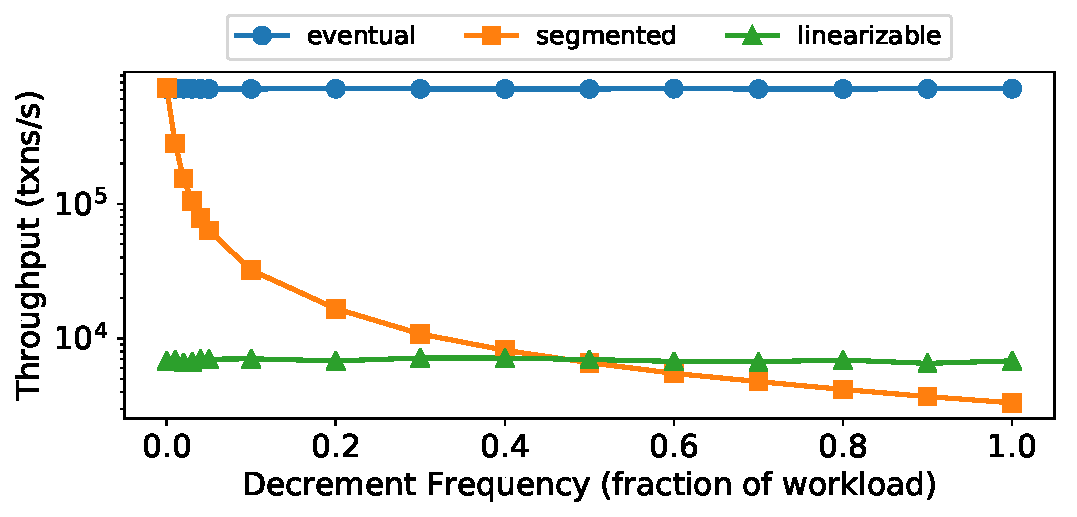
\includegraphics[width=\columnwidth]{figures/vary_withdraws.pdf}
  \end{subfigure}
  \begin{subfigure}[c]{\columnwidth}
    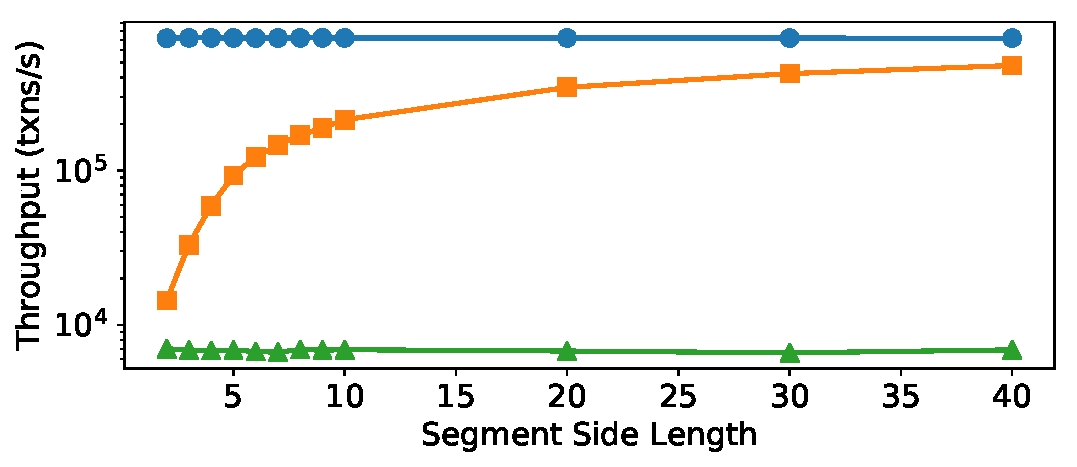
\includegraphics[width=\columnwidth]{figures/vary_segments.pdf}
  \end{subfigure}

  \caption{%
    Segmented invariant-confluent replication throughput versus coordination,
    induced by executing disallowed transactions (top) and by transitioning
    across segments (bottom).
  }\figlabel{ThroughputVsGlobalSyncs}
\end{figure}

\begin{benchmark}\benchlabel{VaryWithdraws}
Consider again the PN-Counter from \exampleref{CounreachableExample} and the
corresponding transactions, invariants, and single-segment segmentation that
forbids concurrent decrements. We replicate this object on 32 servers
deployed on 32 m5.xlarge EC2 instances within the same availability zone.  Each
server has three colocated clients that issue deposit and withdrawal
transactions. We replicate the object with eventual consistency, segmented
invariant-confluence, and linearizability and measure the system's total
throughput as we vary the fraction of client requests that are withdrawals. The
results are shown in the top of \figref{ThroughputVsGlobalSyncs}.

Both eventually consistent replication and linearizable replication are
unaffected by the workload, achieving roughly 700,000 and 7,000 transactions
per second respectively. Expectedly, eventually consistent replication
significantly outperforms linearizable replication because (a) transactions can
be sent to any server (not just the leader) and (b) servers do not coordinate
with each other at all.
%
Segmented invariant-confluent replication performs well for low-withdrawal
workloads and performs increasingly poorly as we increase the fraction of
withdrawal transactions, eventually becoming slower that linearizable
replication. For example, with 5\% withdrawal transactions, segmented
invariant-confluent replication performs an order of magnitude better than
linearizable replication; with 50\% withdrawals, it performs as well; and with
100\% withdrawals, it performs two times worse.

These results are expected. Deposit transactions can execute without any
coordination while withdrawal transactions require global coordination. As we
increase the fraction of withdrawals, we increase the amount of coordination
that the system has to perform which in turn drastically decreases the
throughput. These results also offer two insights:
%
First, for low-withdrawal workloads, segmented invariant-confluent replication
achieves a compromise between strong and weak consistency. It guarantees that
invariants are maintained (which is impossible with eventual consistency if the
object is not invariant-confluent) with performance many times better than
strongly consistent replication.
%
Second, segmented invariant-confluent replication is poorly suited to workloads
that require a large amount of coordination. For workloads without much inherit
concurrency (e.g.\ withdraw-mostly workloads), maintaining invariants is best
done with strong consistency. It provides stronger guarantees with better
performance.
\end{benchmark}

\begin{benchmark}\benchlabel{VarySegmentLength}
  Consider again the object, transactions, and invariants from \exampleref{Z2}
  and \exampleref{SegmentedZ2}. As with \benchref{VaryWithdraws}, we replicate
  the object across 32 servers. Clients issue 50\% increment $x$ transactions,
  and 50\% decrement $y$ transactions. We consider a ``checkerboard''
  segmentation $\Sigma_n = \setst{(I_{i, j}, T)}{i, j \in \ints}$ where segment
  invariant $I_{i, j}$ consists of the square of points $\setst{(x, y)}{ni \leq
  x < n(i + 1), nj \leq y < n(j + 1)}$ with side length $n$. For example,
  $\Sigma_1$ places each point in its own segment, $\Sigma_2$ tessellates
  $\ints^2$ with 2x2 squares, $\Sigma_3$ tessellates $\ints^2$ with 3x3
  squares, and so on. We measure the throughput of the object replicated with
  eventually consistent, segmented invariant-confluent, and linearizable
  replication as we vary the segment side length $n$. The results are shown in
  the bottom \figref{ThroughputVsGlobalSyncs}.

  This benchmark tells the same tale as \benchref{VaryWithdraws}. Eventual
  consistency and linearizability are unaffected by workload, and eventual
  consistency outperforms linearizability by roughly two orders of magnitude.
  In this example, the segmented invariant-confluent replication only requires
  coordination when transitioning between segment boundaries, so as we increase
  the segment side length, the throughput of the system increases
  significantly.
\end{benchmark}

\begin{figure}[ht]
  \centering
  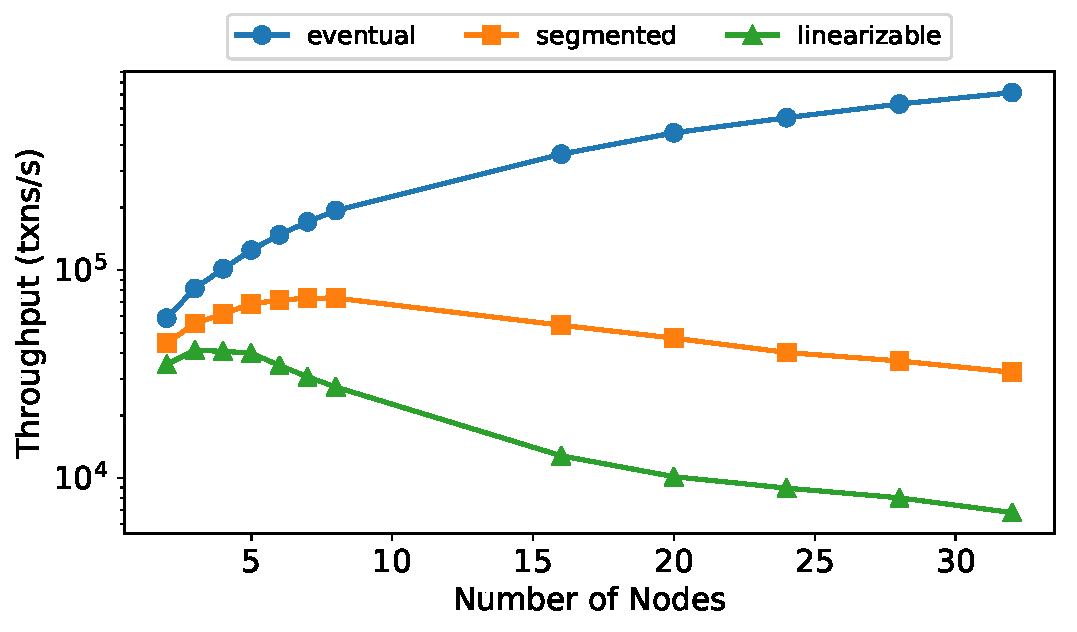
\includegraphics[width=\columnwidth]{figures/vary_nodes.pdf}
  \caption{%
    Throughput of eventually consistent, segmented invariant-confluent, and
    linearizable replication measured against the number of
    nodes.
  }\figlabel{VaryNodes}
\end{figure}

\begin{benchmark}
  In this benchmark, we measure the scale-out of segmented invariant-confluent
  replication. We repeat \benchref{VaryWithdraws} with a 10\% withdrawal rate,
  but this time we vary the number of servers we use to replicate our object.
  When we replicate with $n$ servers, we use $3n$ clients (the $3$ colocated
  clients on each server) as part of the workload. The results are shown in
  \figref{VaryNodes}.

  Eventually consistent replication scales perfectly with the number of nodes,
  confirming the results in~\cite{bailis2014coordination}. With eventually
  consistent replication, servers do not coordinate at all, so they are
  completely unaffected by the number of servers. Linearizable replication, on
  the other hand, scales up to about 3-5 servers before performance begins to
  decrease. These numbers are consistent with typical deployments of
  state-machine replication protocols like Paxos~\cite{chandra2007paxos}.
  Because all messages are sent to the leader, the leader becomes the
  bottleneck as the number of servers and clients increases. Moreover, the
  leader must wait for responses from more servers, increasing the latency of
  the slowest response which in turn decreases throughput.
  Segmented invariant-confluent replication scales up to about 6-8 servers
  before succumbing to the same scalability bottlenecks as linearizable
  replication.

  These results highlight the importance of coordination avoidance in
  distributed databases. While segmented invariant-confluent replication scales
  out slightly better than linearizable replication, both scale significantly
  worse than eventually consistent replication even for a very low (i.e.\ 10\%)
  withdrawal workload. This demonstrates that even a small amount of
  coordination can significantly reduce the scalability of a system.
\end{benchmark}
}
\end{document}
